\documentclass[11pt,a4paper]{report}

\title{Appunti del corso di Statistica Matematica}
\author{Gadotti Andrea, Nardin Michele, Peruzzetto Marco}
\date{}

\usepackage{amsmath}%
\usepackage{bbm}%
\usepackage[utf8]{inputenc}
\usepackage[italian]{babel}
\usepackage{longtable}
\usepackage{amsthm}
\usepackage{amscd}
\usepackage{amssymb}
\usepackage{amsfonts}
\usepackage{amsmath}
\usepackage{mathtools}
\usepackage{enumitem}
\usepackage{vmargin}
\usepackage[scale=3]{ccicons}
\usepackage{hyperref}
%\usepackage{graphicx}


\newtheorem{corollario}{Corollario}
\newtheorem{oss}{Osservazione}
\newtheorem{definizione}{Definizione}
\newtheorem{esempio}{Esempio}
\newtheorem{proposizione}{Proposizione}
\newtheorem{teo}{Teorema}
\newtheorem*{theorem}{Teorema}
\newtheorem*{lemma}{Lemma}

\newcommand{\ud}{\,\mathrm{d}}
\DeclareMathOperator{\im}{im}
\DeclareMathOperator{\ri}{Risk}
\DeclareMathOperator{\ggt}{ggT}
\DeclareMathOperator{\mse}{MSE}
\DeclareMathOperator{\eendd}{End}
\DeclareMathOperator{\tr}{tr}
\DeclareMathOperator{\lo}{Loss}
\DeclareMathOperator{\dom}{Dom}
\DeclareMathOperator{\id}{id}
\DeclareMathOperator{\bi}{Bin}
\DeclareMathOperator{\sign}{sign}
\DeclareMathOperator{\uni}{Unif}
\DeclareMathOperator{\rg}{rg}
\DeclareMathOperator{\homm}{Hom}
\DeclareMathOperator{\iso}{Iso}
\DeclareMathOperator{\asin}{asin}
\DeclareMathOperator{\acos}{acos}
\DeclareMathOperator{\supp}{supp}
\DeclareMathOperator{\var}{Var}
\DeclareMathOperator{\ar}{arg}
\DeclareMathOperator{\eff}{eff}
\DeclareMathOperator{\cova}{Cov}


\providecommand{\abs}[1]{\lvert#1\rvert}
\providecommand{\Abs}[1]{\bigg\lvert#1\bigg\rvert}
\providecommand{\norm}[1]{\lVert#1\rVert}



\begin{document}
\setpapersize{A4}
\setmarginsrb{35mm}{20mm}{25mm}{35mm}%
             {0mm}{10mm}{0mm}{10mm}
             
\maketitle

\pagenumbering{gobble}
\null
\vfill
\noindent \ccbysa  \\
\\
\textbf{Quest'opera è distribuita con Licenza Creative Commons Attribuzione - Condividi allo stesso modo 3.0 Italia.} \\
Per leggere una copia della licenza visita il sito web \url{http://creativecommons.org/licenses/by-sa/3.0/it/} o spedisci una lettera a Creative Commons, 171 Second
Street, Suite 300, San Francisco, California, 94105, USA.


\newpage
\pagenumbering{arabic}

\tableofcontents
\chapter{Prima parte del corso}
\section{Introduzione}
%%%%lezione 18 febbraio%%%%

\subsection{Funzione generatrice dei momenti}
Lezione del 18/02, ultima modifica 04/03, Andrea Gadotti

\begin{definizione}
Sia $X$ una variabile casuale (discreta o assolutamente continua). Se esiste $t_0 > 0$ tale per cui $\mathbbm{E}(e^{tX}) < +\infty$ $\forall t \in (-t_0 , t_0)$, chiameremo la funzione 

$$M_X := \mathbbm{E}(e^{tX})$$
funzione generatrice dei Momenti di $X$.
\end{definizione}
\textbf{Esempi}
\begin{enumerate}
\item $X \sim b(1,p)$ con $p \in (0,1)$. Si ha:

$$M_X (t) 	= \mathbbm{E}(e^{tX}) 
			= \displaystyle\sum_{x=0}^1 e^{tx} \mathbbm{P}(X=x)$$
$$
			= \displaystyle\sum_{x=0}^1 e^{tx} p^x (1-p)^{1-x}
			= p e^t + (1-p)$$	


\item $X \sim P(\lambda)$ con $\lambda > 0$. Si ha:

$$M_X (t) 	= \mathbbm{E}(e^{tX}) 
			= \displaystyle\sum_{x=0}^{+\infty} e^{tx} \frac{e^{-\lambda} \lambda^x}{x!}
			= e^{\lambda (e^t -1)}$$
			
			
\item $X \sim G(\alpha, \beta)$, ovvero 

$$f_X (x; \alpha, \beta) := \frac{1}{\Gamma (\alpha) \beta^{\alpha}} x^{\alpha -1} e^{-\frac{1}{\beta} x}$$ con $\alpha>0$, $\beta>0$, $x>0$ e 

$$\Gamma(\alpha) := \int_0^{+\infty} \! x^{\alpha -1} e^{-x} \mathrm{d}x$$ 

(nota: $\alpha \in \mathbbm{N} \Longrightarrow \Gamma(\alpha)=(\alpha - 1)$)

Abbiamo che: 

$$M_X (t)	= \mathbbm{E}(e^{tX})
			= \int_0^{+\infty} \! e^{tx} \frac{1}{\Gamma (\alpha) \beta^{\alpha}} x^{\alpha -1} e^{-\frac{1}{\beta} x} \mathrm{d}x$$
\begin{center} $=$ ...[sostituzione $\sigma := x(\frac{1}{\beta} - t)$]...  \end{center}
			$$= \frac{1}{(1-\beta t)^{\alpha}}$$ con $t < \frac{1}{\beta}$
			
\end{enumerate}

\paragraph{Momenti di una variabile casuale}

\begin{definizione}
Se una variabile casuale ammette FGM derivabile infinite volte in un intorno di $t=0$ e se tutti i suoi momenti sono finiti, allora definiamo il momento di ordine $s$ non centrato: 
$$\mu'_s := \mathbbm{E} (X^s) = \frac{d^s}{dt^s} M_X (t) \! \mid_{t=0}$$ 
Il momento di di ordine $s$ centrato in $a \in \mathbbm{R}$ è: 

$$\mu_s (a) := \mathbbm{E} ((X-a)^s)$$
Ovvero $\mu'_s = \mu_s (0)$. E' chiaro che $\mu'_1 = \mathbbm{E} (X)$.
Chiameremo infine momento di ordine $s$ centrato (senza specificare altro, intenderemo centrato in $\mu'_1$):

$$\mu_s := \mathbbm{E} ((X-\mu'_1)^s)$$
\end{definizione}

\begin{teo}
Vale la seguente relazione tra momenti centrati e non:
$$\mathbbm{E} ((X-\mu'_1)^s) = \displaystyle\sum_{m=0}^s (-1)^m \binom{s}{m} \mu'_{s-m} (\mu'_1)^m$$
\end{teo}

Osserviamo che $\mu_2 = \mathbbm{E} ((X-\mu'_1)^2) = Var(X) = \mathbbm{E} (X^2) - (\mathbbm{E} (X))^2 = \mu'_2 - (\mu'_1)^2$


\begin{teo}
Date due (o più) v.c. $X$ e $Y$ aventi $f$ densità / $f$ massa $f_X$ e $f_Y$ e fgm $M_X(t)$ e $M_Y(t)$ rispettivamente e assunte $X$ e $Y$ essere indipendenti, allora si ha

$$M_{X+Y} = M_X(t) M_Y(t)$$
\end{teo}

\begin{teo}
Siano $X$ e $Y$ v.c. con funzioni di ripartizione $F_X(x)$ e $F_Y(y)$ rispettivamente. Siano $M_X(t)$ e $M_Y(t)$ le fgm di $X$ e $Y$. Se $M_X(t) = M_Y(t)$ per ogni $t$ in un intorno dell'origine, allora 

$$X \stackrel{d}{=} Y$$
\end{teo}

\begin{oss}
Il teorema appena visto ci dice sostanzialmente che, se esiste, la fgm caratterizza la distribuzione della corrispondente v.c.
\end{oss}
\textbf{Esempio}
Siano $(X_1,...,X_n)$ risultati della replicazione di un esponenzionale casuiale dicotomico $(X_i \sim b(1,p))$. Vogliamo trovare la distribuzione di $S_n := \displaystyle\sum_{i=1}^n X_i$. Calcoliamo quindi la sua fgm:

$$M_{S_n}(t) = \mathbbm{E}({e^{tS_n}}) = \mathbbm{E}({e^{t \sum_{i=1}^n X_i}}) $$
$$\stackrel{TEO 1}
{=} \displaystyle\prod_{i=1}^n \mathbbm{E}({e^{tX_i}}) = \displaystyle\prod_{i=1}^n M_{X_i}(t) = \displaystyle\prod_{i=1}^n (p e^t + (1-p)) = (p e^t + (1-p))^n$$ ovvero $S_n$ è distribuita come $b(n,p)$ per il Teorema 2.

\textbf{esercizio}
Ripetere il calcolo precedente supponendo $X_i \sim P(\lambda), \forall i$.

\subsection{Famiglia Esponenziale a $k$ parametri}
Una famiglia di $f$ densità / $f$ massa è detta essere una Famiglia Esponenziale a $k$ parametri $\theta_1,...,\theta_k$ se la corrispondente $f$ densità / $f$ massa (che è indicizzata da $\theta_1,...,\theta_k$) può essere scritta come

$$f_X(x;\theta) = C^*(x) D^*(\theta) \lbrace \displaystyle\sum_{m=1}^k A_m(\theta) B_m (x) \rbrace$$

dove $C^*(x)$ è una funzione della sola $x$, $D^*(\theta)$ è una funzione del solo $\theta$, $A_m(\theta)$ è una funzione del solo $\theta$ e $B_m(x)$ è una funzione della sola $x$.
\textbf{Esempi}
\begin{enumerate}
\item 
$X \sim G(\alpha, \beta) \Longrightarrow f_X(x; \alpha, \beta) = \frac{1}{\Gamma(\alpha) \beta^\alpha} x^{\alpha -1} e^{- \frac{1}{\beta} x} \mathbbm{1}_{\mathbbm{R}^+}(x)$, $\alpha >0$, $\beta >0$
$\mathbbm{1}_{\mathbbm{R}^+}$ è detto supporto della distribuzione.
Quindi possiamo riscrivere $f_X(x; \alpha, \beta)$ come
$$f_X(x; \alpha, \beta) = \frac{1}{\Gamma(\alpha) \beta^\alpha} \mathbbm{1}_{\mathbbm{R}^+}(x) exp((\alpha -1) ln(x) - \frac{1}{\beta} x)$$
e quindi ponendo $D^*(\alpha, \beta) := \frac{1}{\Gamma(\alpha) \beta^\alpha}$, $C^*(x) := \mathbbm{1}_{\mathbbm{R}^+}(x)$, $A_1(\alpha, \beta) := (\alpha -1)$, $B_1(x) := ln(x)$, $A_2(\alpha, \beta) := - \frac{1}{\beta}$ e $B_2(x) := x$, otteniamo $G(\alpha, \beta)$ come famiglia esponenziale con $k=2$.

\item $X \sim b(n,p) \Longrightarrow f_X(x; n,p) = \binom{n}{x} p^x (1-p)^{n-x} \mathbbm{1}_{\lbrace 0,1,...,n \rbrace}(x)$ con $n \in \mathbbm{N}$ noto.
Quindi possiamo riscrivere $f_X(x; n,p)$ come
$$f_X(x; n,p) = \binom{n}{x} \mathbbm{1}_{\lbrace 0,1,...,n \rbrace}(x) (1-p)^n exp(ln(\frac{p}{1-p}) x)$$ con $\frac{p}{1-p}$ detto odd ratio o parametra naturale della famiglia esponenziale.\\
Quindi ponendo $D^*(p) := (1-p)^n$, $C^*(x) := \binom{n}{x} \mathbbm{1}_{\lbrace 0,1,...,n \rbrace}(x)$, $A_1(p) := ln(\frac{p}{1-p})$, $B_1(x) := x$, otteniamo $b(n,p)$ come famiglia esponenziale con $k=1$.
\end{enumerate}

\begin{oss}
Le famiglie di esponenziali di ?...? hanno interessanti proprietà matematiche (proprietà di regolarità).

Dal punto di vista statistico, ciò si traduce in un'interessante conseguenza: tutta l'informazione contenuta nei dati a disposizione $(X_1,...,X_n)$ relativa alla funzione $f_X (x; \theta)$ può essere sintetizzata attraverso $k$ quantità (funzioni di $(X_1,...,X_n)$) che potranno essere impiegate per costruire procedure inferenziali (stima, test per la verifica di ipotesi) riguardanti il parametro $\theta$.\\
Ovvero, l'appartenenza a una famiglia esponenziale permette una riduzione dei dati $(X_1,...,X_n)$ via $B_m$.\end{oss}
%%%%lezione 1 marzo%%%%

\subsection{Trasformazioni di variabili casuali}
Lezione del 01/03, ultima modifica 03/03
\paragraph{Discrete}
\begin{teo}
Sia X una vc con funzione di massa $f_X(x)=P(X=x)$, e sia $A_X$ il suo supporto. 
Sia W=h(X) una nuova vc. Allora $$P(W=w)=\sum_{\{x\in A_X:h(x)=w\}}P(X=x)$$
\end{teo}

\textbf{Esempi}
\begin{enumerate}

\item Sia $X \sim b(n,p)$ con relativa funzione di massa 
$f_X(x,p)=\binom{n}{p}p^x(1-p)^{n-x}\mathbbm{1}_{0,1,...,n}(x)$,
$n$ noto e $p\in(0,1)$.

Considero quindi $W=n-X$. Come si distribuisce $W$? 
$$P(W=w)=P(X=n-w)=\binom{n}{n-w}p^{n-w}(1-p)^w\mathbbm{1}_{0,1,...,n}(w)$$
\item Sia $X$ una vc tale che 
$f_X(x)=P(X=x)=\left(\frac{1}{2}\right)^x\mathbbm{1}_\mathbbm{N}(x)$, $W=X^3$. 
%%lasciando una riga vuota va a capo senza dare badbox! figata
$$P(W=w)=P(X^3=w)=P(X=\sqrt[3]{w})=\left(\frac{1}{2}\right)^{\sqrt[3]{w}}\mathbbm{1}_{1,8,27,...}(w)$$
\end{enumerate}

\paragraph{Assolutamente continue}
\begin{teo}
Sia X una variabile casuale (ass continua) con funzione di densità $f_X(x)$ e sia $W=h(X)$, ove $h$ è una funzione monotona. 
Supponiamo inoltre che $f_X(x)$ sia continua sul supporto di X e che $h^{-1}(w)$ abbia derivata continua sul supporto di W. Allora
$$f_W(w)=f_X(h^{-1}(w))\left|\frac{d}{dw}h^{-1}(w)\right|\mathbbm{1}_{A_W}(w)$$
\end{teo}
\textbf{Esempio}
(Standardizzazione di una vc normale)
Sia $X \sim N(m,s^2)$. 
Considero $W=h(X)=\frac{X-m}{s}$. 
Allora, dato che $h^{-1}(w)=sw+m$, 
che ha derivata continua su tutto $\mathbbm{R}$,  
$$f_W(w)=f_X(sw+m)|s|=\frac{e^{\frac{-w^2 }{2}}}{\sqrt{2\pi}}$$
\begin{teo}
Se $W=h(X)$ ove h è monotona a tratti (un numero finito k) e valgono le condizioni del teorema precedente (su ogni tratto), allora
$$f_W(w)=\sum_{n=1}^k f_X(h_n^{-1}(w))\left|\frac{d}{dw}h_n^{-1}(w)\right|\mathbbm{1}_{A_W}(w)$$
\end{teo}
\textbf{Esempio} (Chi-quadro): Sia $X \sim N(0,1)$ e $W=h(X)=X^2$. $h$ è monotona sui tratti $A_0={0}$, $A_1=(-\infty,0)$, $A_2=(0,+\infty)$. 
Trovo inoltre $h_1^{-1}(w)=-\sqrt{w}\in A_1 \forall w \geq 0$, mentre $h_2^{-1}(w)=\sqrt{w}\in A_2 \forall w \geq 0$. 
$\frac{d}{dw} h_1^{-1}(w)=-\frac{1}{2\sqrt{w}}$, $\frac{d}{dw} h_2^{-1}(w)=\frac{1}{2\sqrt{w}}$ sono entrambe continue su $\mathbbm{R}_+$.
$$f_W(w)=\frac{1}{\sqrt{2\pi}}e^{\frac{-(-\sqrt{w})^2 }{2}}\left|\frac{1}{2\sqrt{w}}\right|+\frac{1}{\sqrt{2\pi}}e^{\frac{-(\sqrt{w})^2 }{2}}\left|\frac{1}{2\sqrt{w}}\right|$$ 
$$=\frac{1}{\sqrt{2\pi w}}
e^{\frac{-w}{2}}\mathbbm{1}_{\mathbbm{R}+}
(w)=\frac{1}{2^{1/2}\Gamma(1/2)}
w^{\frac{1}{2}-1}e^{\frac{-w}{2}}$$
Si riconosce che $W \sim \mathcal{G}(\alpha=1/2,\beta=2)$ e si chiama Chi quadrato con $\nu=1$ gradi di libertà.
In generale, una vc Chi Quadro con $\nu=n$ gradi di libertà è $W=\sum_{i=1}^n X_i^2$, ove $X_1,X_2,...,X_n$ sono vc iid N(0,1). Per il teorema sulla FGM di una somma di vc iid si trova immediatamente che $W \sim \mathcal{G}(\alpha=n \cdot 1/2,\beta=2)$.
\subsection{Convergenze}
\paragraph{Convergenza in probabilità}
\begin{definizione}

Sia $\{X_n\}_{n\in\mathbbm{N}}$ una successione di variabili casuali e 
sia X un'altra variabile casuale, tutte definite sullo stesso spazio campionario.
Diciamo che $X_n$ converge in probabilità a X (scriviamo $X_n\stackrel{p}{\rightarrow}X$) se $\forall\varepsilon>0$ $$\lim_{n \rightarrow\infty} P(|X_n-X|\leq\varepsilon)=0$$
\end{definizione}
\begin{oss}
Se $X_n\stackrel{p}{\rightarrow}X$ diciamo che la "massa" della differenza $|X_n-X|$ converge a 0.
Inoltre, quando scriviamo $X_n\stackrel{p}{\rightarrow}X$, stiamo sottintendendo tutta la parte iniziale della definizione precendete, cioè il "sia $\{X_n\}_{n\in\mathbbm{N}}$ una successione di variabili casuali...".
\end{oss}
\begin{teo} Alcuni risultati utili: 

\begin{enumerate}
\item Supponiamo che  $X_n\stackrel{p}{\rightarrow}X$ e  $Y_n\stackrel{p}{\rightarrow}Y$. Allora  $X_n+Y_n\stackrel{p}{\rightarrow}X+Y$
\item Supponiamo che $X_n\stackrel{p}{\rightarrow}X$ e sia a una costante. Allora $aX_n\stackrel{p}{\rightarrow}aX$ 
\item Supponiamo che  $X_n\stackrel{p}{\rightarrow}a$ costante, e sia g una funzione reale continua in a. Allora  $g(X_n)\stackrel{p}{\rightarrow}g(a)$
\item (Corollario di 3.) Se $X_n\stackrel{p}{\rightarrow}a$, allora $X_n^2\stackrel{p}{\rightarrow}a^2$, $\frac{1}{X_n}\stackrel{p}{\rightarrow}\frac{1}{a}$ (se $a\neq0$), $\sqrt{X_n}\stackrel{p}{\rightarrow}{a}$ ($a\geq0$).
\item $X_n\stackrel{p}{\rightarrow}X$ e $Y_n\stackrel{p}{\rightarrow}Y$ allora $X_nY_n\stackrel{p}{\rightarrow}XY$
\end{enumerate}
\end{teo}
%\textbf{Esempi}
%\begin{enumerate}
%\item
%\item
%\item
%\end{enumerate}
\paragraph{Convergenza in distribuzione}
\begin{definizione}

Sia $\{X_n\}_{n\in\mathbbm{N}}$ una successione di variabili casuali e 
sia X un'altra variabile casuale, tutte definite sullo stesso spazio campionario.

Siano $F_{X_n}$ e $F_X$ le relative funzioni di ripartizione (di distribuzione, sinonimo).
Sia $C(F_X)$ l'insieme dei punti ove $F_X$ è continua. 
Diciamo che $X_n$ converge in distribuzione (o in legge) a X (scriviamo $X_n\stackrel{d}{\rightarrow}X$) se 
$$\lim_{n \rightarrow\infty} F_{X_n}(x)=F_X(x) \forall x \in C(F_X)$$
\end{definizione}
\textbf{Esempio}
\begin{teo}
Se $X_n\stackrel{p}{\rightarrow}X$ allora $X_n\stackrel{d}{\rightarrow}X$.
\end{teo}
\begin{oss}
Il contrario in generale non vale, tranne nel caso in cui X è una vc degenere (cioè costante).
\end{oss}
\begin{teo} Supponiamo che $X_n\stackrel{d}{\rightarrow}X$ e sia g una funzione continua sul supporto di X. Allora $g(X_n)\stackrel{d}{\rightarrow}g(X)$
\end{teo}
\begin{teo} [Slutsky] Supponiamo che $X_n\stackrel{d}{\rightarrow}X$, $A_n\stackrel{p}{\rightarrow}a$ costante e $B_n\stackrel{p}{\rightarrow}b$ costante. Allora $A_n+B_n X_n\stackrel{d}{\rightarrow}a+bX$
\end{teo}
%%%%fine lezione del 1 marzo%%%%
\subsection{Teoria asintotica}
Lezione del 04/03, ultima modifica 05/03

\begin{teo}
\noindent
($\Delta$-method) Sia $\{X_n\}_{n \in\ \mathbbm{N}}$ una successione di vc
tale che 

\noindent $\sqrt{n}(X_n-\vartheta)\stackrel{d}{\rightarrow}N(0,\sigma^2)$. 
Supponiamo che una funzione g(X) sia derivabile in $\vartheta$ e che $g'(\vartheta)\neq0$. Allora $$\sqrt{n}(g(X_n)-g(\vartheta))\stackrel{d}{\rightarrow}N(0,\sigma^2(g'(\vartheta))^2)$$
\end{teo}

\textbf{Esempi}
\begin{enumerate}
\item Considero $$Y_n=\frac{\chi^2_n-n}{\sqrt{2n}}=\sqrt{n}\left(\frac{\chi^2_n}{\sqrt{2}n}-\frac{1}{\sqrt{2}}\right)$$ ove $\chi^2_n$ è la chiquadro con n gradi di libertà. 
Ricordiamo che $\mathbbm{E}(\chi^2_n)=n$ e che $Var(\chi^2_n)=2n$ (discende dal fatto che $\chi^2_n \sim \mathcal{G}(\alpha=n/2,\beta=2)$. 
Siccome $Y_n \stackrel{d}{\rightarrow} N(0,1)$, scrivendo $Y_n$ nella forma $Y_n=\sqrt{n}\left(\frac{\chi^2_n}{\sqrt{2}n}-\frac{1}{\sqrt{2}}\right)$ riconosciamo che la prima parte delle ipotesi del $\Delta$-method sono soddisfatte.
Considero quindi $g(t)=\sqrt{t}$, che è derivabile in $\vartheta=1/\sqrt{2}$, $g'(t)=\frac{1}{2\sqrt{t}}|_{\vartheta=1/\sqrt{2}}=2^{-3/4}$.
Allora $$\sqrt{n}(g\left(\frac{\chi^2_n}{\sqrt{2}n}\right)-g(\vartheta))=
\sqrt{n}\left(\sqrt{\frac{\chi^2_n}{\sqrt{2}n}}-\sqrt{\frac{1}{\sqrt{2}}}\right)
\stackrel{d}{\rightarrow}N(0,1^2\cdot 2^{-3/2})$$
\end{enumerate}

\begin{teo}
(Teorema centrale del limite) Siano $X_1,...X_n$ vc iid dotate di media $\mu$ e varianza finita $\sigma^2$. Allora 
$$\frac{\sum_{i=1}^n X_i - n\mu}{\sqrt{n}\cdot \sigma} = \frac{\sqrt{n}(\bar{X_n}-\mu)}{\sigma}\stackrel{d}{\rightarrow}N(0,1) $$
\end{teo}

\textbf{Esempi/Applicazioni}
\begin{enumerate}
\item $X \sim b(n,p)$, $X \stackrel{a}{\sim}N(np,np(1-p))$
\item $X_1,...,X_n$ vc 
$P(\lambda =1)$. 
Considero $Y_n=\sum X_i$.
Dato che $Y_n \stackrel{a}
{\sim} N(n\lambda ,n \lambda )$,
 $\frac{Y_n}{n} \stackrel{a}
 {\sim} N(1,1/n)$
\item Considerato $W_n=\sqrt{n}(Y_n/n-1)=\frac{Y_n/n-1}
{1/\sqrt{n}}=\frac{\bar{Y_n} - \mathbbm{E}(\bar{Y_n})}
{\sqrt{Var(Y_n/n)}}$
\end{enumerate}

\begin{teo}
Sia $\{X_n\}$ una succ di vc iid con FGM $M_{X_n}(t)$ definita e $<\infty$ per $t\in(-h,h) \forall n$, e sia X un'altra vc con FGM $M_X(t)$ definita e $<\infty$ per $t \in (-h_1,h_1), h_1\leq h$. Se $$\lim_{n \rightarrow +\infty} M_{X_n}(t)=M_X(t) \forall |t| \leq h_1$$ allora $X_n \stackrel{d}{\rightarrow} X$.
\end{teo}
\textbf{Applicazione}

Sia $X_n \sim b(n,p)$. 
Ricordiamo che $X_n=\sum X_i$ ove $X_i \sim b(1,p)$, ed inoltre $\mu=\mathbbm{E}(X)=np$.
Siccome $M_{X_n}(t)=
\mathbbm{E}(e^{tX_n})=[(1-p)+pe^t]^n=
[1+\frac{\mu}{n}(e^t - 1)]^n$, 
$$ M_{X_n}(t) \stackrel{n \rightarrow \infty}{\longrightarrow} 
e^{\mu(e^t-1)}$$
che è la FGM di una Poisson di parametro $\mu$.

\section{Approccio alla Statistica Matematica}

\subsection{Introduzione}

\begin{definizione} (Campione Casuale)
Il vettore casuale $(X_1,...,X_n)$ si dice Campione Casuale relativamente ad una vc $X \sim F_X(x,\vartheta)$ se i suoi elementi sono vc i.i.d.
\end{definizione}
\textbf{Osservazione}
Il fatto che le vc siano i.i.d. implica che $$F_{X_1,...,X_n}(X_1,...,X_n)=\prod_{i=1}^n F_{X_i} (X_i)$$ e $$f_{X_1,...,X_n}(X_1,...,X_n)=\prod_{i=1}^n f_{X_i} (X_i)$$

\begin{definizione} (Statistica)
Sia $(X_1,...,X_n)$ un campione casuale da una distribuzione associata alla vc $X$, e sia $\Omega$ lo spazio campionario di $(X_1,...,X_n)$

\noindent Ogni funzione $$T(X_1,...,X_n):\Omega \longrightarrow \mathbbm{R}^k$$ che NON dipende da parametri incogniti è detta Statistica.
\end{definizione}

\textbf{Osservazioni}
Le cose scritte tra virgolette "" sono concetti e/o definizioni non ancora introdotti, che vengono usati per dare un'idea intuitiva di quello che si andrà a vedere, cose che poi durante il corso verranno trattate con rigore.
\begin{enumerate}
\item Una statistica T è una "caratteristica numerica" del campione: si presta a $sintetizzare$ l'informazione su $\vartheta$ contenuta nel campione.
\item $\sum_{i=1}^n X_i$ e $\sum_{i=1}^n X_i^2$ sono entrambe statistiche: sono alla base di due "stimatori" molto importanti:

Media Campionaria: $\bar{X}_n =\frac{1}{n}\sum X_i$

Varianza Campionaria: $S_n^2=\frac{1}{n-1} \sum (X_i-\bar{X}_n)^2 = \frac{1}{n-1} \sum X_i^2 - \frac{n}{n-1}\bar{X}_n^2$
\item Ogni statistica è una vc: ha quindi una distribuzione, che dipende dal parametro.

\textbf{Esempio} Considero $\bar{X}=\frac{1}{n} \sum X_i$ ove $X_i \sim N(\mu,\sigma^2)$. Allora $\bar{X} \sim N(\mu,\frac{\sigma^2}{n})$. Da questo si potrà dedurre la "bontà" di $\bar{X}$ come "stimatore" di $\mu$.
\item Tra tutti i modi di sintetizzare l'informazione contenuta in $(X_1,...,X_n)$ relativamente a $\vartheta$, siamo interessati a quelli che NON tralasciano informazioni o quote di informazioni rilevanti per il parametro.
\item In relazione ad uno stimatore potremmo essere interessati ad alcune proprietà, in particolare a queste due:

$\cdot$ Accuratezza [concetto legato alla media dello stimatore] ($Non$ $distorsione$)

$\cdot$ Precisione [concetto legato alla varianza dello stimatore] ($efficienza$ o $consistenza$)
\end{enumerate}
%Fine lezione del 4 marzo. ultima modifica 5 marzo, 14.08, Michele
\subsection{Statistiche d'ordine}
Lezioni 08 e 11 Marzo, ultima modifica 21/03, Scritte da: Marco Peruzzetto

\textbf{Definizione.} Sia $\left(X_1,\ldots ,X_n\right)$ un campione casuale con distribuzione $F_X\left(x,\theta\right)$, densità $f_X\left(x,\theta\right)$ e supporto $\supp\{X\}\coloneqq (a,b)\subset\mathbb{R}$ ove $X\in \{X_1,\ldots,X_n\}$ e $-\infty\leq a<b\leq +\infty$. Definiamo ricorsivamente le seguenti variabili casuali:
\begin{itemize}
\item $X_{(1)}\coloneqq \min\left(\{X_1,\ldots,X_n\}\right)$;
\item $X_{(i)}\coloneqq \min\left(\{X_1,\ldots,X_n\}\setminus\{X_{(1)},\ldots,X_{(i-1)}\}\right)$ $\forall 1<i\leq n$. 
\end{itemize}
Chiameremo allora $X_{(i)}$ la $i$-esima \textit{Statistica d'Ordine} del campione.\\
\textit{Osservazione:} La statistica d'ordine consiste semplicemente nel vettore per il quale le variabili casuali vengono appunto ordinate, in base al valore che assumono in un determinato punto del loro dominio comune, in ordine crescente. In particolare $X_{(i)}$ sarà l' $i$-esima variabile più piccola. Naturalmente, se il campione ha lunghezza $n$, allora $X_{(n)}=\max\left(\{X_1,\ldots,X_n\}\right)$. 
Osserviamo che la funzione $\left(X_1,\ldots,X_n\right)\longmapsto \left(X_{(1)},\ldots,X_{(n)}\right)$ è essa stessa una Statistica.
\begin{theorem}
Sia $\left(X_1,\ldots,X_n\right)$ un campione casuale come sopra. Allora si ottiene $\forall$ $1\leq m\leq n$ che la densità dell' $m$-esima statistica d'ordine è data da: 
\begin{displaymath}
f_{X_{(m)}}\left(x,\theta\right)=\frac{n!}{(m-1)!(n-m)!}f_X\left(x,\theta\right)\cdot F_X\left(x,\theta\right)^{m-1}\cdot \big(1-F_X\left(x,\theta\right)\big)^{n-m}
\end{displaymath}
\end{theorem}
Daremo due dimostrazioni, la seconda più bella della prima.
\begin{proof} Innanzi tutto si ha che il supporto $(a,b)$ può essere partizionato in $n$ parti, per cui evidentemente si ha: 
\footnotesize{
\begin{displaymath}
f_{(X_{(1)},\ldots,X_{(n)})}(x_{(1)},\ldots,x_{(n)},\theta)=
\left\{
\begin{array}{lr}
n!\prod_{i=1}^n f_{X}(x_{(i)},\theta) & \mbox{se } a<x_{(1)}<x_{(2)}<\ldots <x_{(n)}<b \\
0 & \mbox{altrimenti.}
\end{array}
\right.
\end{displaymath}
} \normalsize{ove la produttoria è giustificata dal fatto che le variabili sono tutte indipendenti e che devono essere ciascuna minore dell'altra per l'ordinamento assegnato; il coefficiente fattoriale è presente poiché le $n$ parti dell'intervallo $(a,b)$ possono essere assegnate alle $n$ variabili in tale numero di modi, dato che ciascuna $X_i$ $\forall 1\leq i\leq n$ ha la stessa distribuzione.  \\ Adesso per trovare la distribuzione di ciascuna $X_{(m)}$ sarà dunque sufficiente integrare $f_{(X_{(1)},\ldots,X_{(n)})}$ nei domini possibili di tutte le altre funzioni di distribuzione di ciascuna $X_{(i)}$ con $i\neq m$. In particolare, ciascuna $f_{X_{(i)}}$ per $i<m$ dovrà assumere a piacere valori necessariamente inferiori a $f_{X_{(m)}}$, viceversa ogni $f_{X_{(i)}}$ per $i>m$ dovrà assumere valori obbligatoriamente superiori a quelli di $f_{X_{(m)}}$ in ogni punto. Ricordando allora che possiamo scrivere la distribuzione come $\int_a^x f_X(\theta,t)dt=F_X(\theta,x)$ essendo la densità la derivata della funzione di distribuzione, otterremo quindi che $\forall a<x_{(m)}<b$ la distribuzione sarà data da: \\\\ $f_{X(m)}(x_{(m)},\theta)=$	}
\small{
\begin{eqnarray*}
&=&\int_a^{x_{(2)}} dx_{(1)}\cdots\int_a^{x_{(m)}} dx_{(m-1)}\int_{x_{(m)}}^b dx_{(m+1)}\cdots\int_{x_{(n-1)}}^b dx_{(n)}f_{(X_{(1)},\ldots,X_{(n)})}(x_{(1)},\ldots,x_{(n)},\theta)\\
&=&\int_a^{x_{(2)}} dx_{(1)}\cdots\int_a^{x_{(m)}} dx_{(m-1)}\int_{x_{(m)}}^b dx_{(m+1)}\cdots\int_{x_{(n-1)}}^b dx_{(n)} n!\prod_{i=1}^n f_{X}(x_{(i)},\theta) \\
&=& f_{X}(x_{(m)})\int_a^{x_{(2)}} dx_{(1)}\cdots\int_a^{x_{(m)}} dx_{(m-1)}\int_{x_{(m)}}^b dx_{(m+1)}\cdots\int_{x_{(n-1)}}^b dx_{(n)} n!\prod_{i=1,i\neq m}^n f_{X}(x_{(i)},\theta) \\
&=& \frac{n!}{(m-1)!(n-m)!}f_X\left(x,\theta\right)\cdot F_X\left(x,\theta\right)^{m-1}\cdot \big(1-F_X\left(x,\theta\right)\big)^{n-m}, 
\end{eqnarray*}
}
\normalsize{dove è stato usato il fatto che $\int_a^b F_X^\alpha(\theta, t)f_X(\theta,t)dt=\frac{F_X^{\alpha+1}}{\alpha+1}$, $\forall \alpha\neq -1$.}
\end{proof} 

\begin{proof}
Sia $\Omega$ il dominio comune del campione casuale. Definiamo per $x\in \mathbb{R}$ la nuova variabile casuale $Y_x$ come:
\begin{align*}
\Omega &\longrightarrow  \{0,\ldots,n\} \\
Y_x(\omega)  &\coloneqq   \sum_{i=1}^n \mathbbm{1}_{\{X_i(\omega)\leq x\}}(\omega)=\#\big\{i\in\{1,\ldots,n\}: X_i\leq x\big\},
\end{align*}
funzione che, per così dire, ``conta'' il numero di variabili casuali $X_i$ che non superano $x$. Si vede immediatamente che $\forall 1\leq m\leq n$, si ha la distribuzione 
\begin{eqnarray*}
F_{X_{(m)}}(\theta,x) &=& \mathbb{P}[Y_x\geq m]=\sum_{k=m}^n \mathbb{P}[Y_x=k]= \\
&=& \sum_{k=m}^n \binom{n}{k}F_X^k(\theta,x)\big(1-F_X(\theta,x)\big)^{n-k}.
\end{eqnarray*}
Come nella prima dimostrazione usiamo il fatto che la densità si può vedere come derivata della funzione di ripartizione. Ne segue che per calcolare la densità sarà sufficiente calcolare la derivata in ciascun punto $x$ della distribuzione appena trovata. In particolare si potrà vedere che coesisteranno il termine che vogliamo ottenere con altre due sommatorie, che tuttavia si elidono l'una con l'altra lasciando quindi la relazione espressa dal teorema. Si ha infatti che: 
\\
\small{
\begin{equation*}\label{e:barwq}\begin{split}
f_{(m)}(\theta,x)&=\frac{\partial}{\partial x}F_{X_{(m)}}(\theta,x)= \\
&=\sum_{k=m}^n \binom{n}{k}\cdot f_{X}(\theta,x) \bigg\{k F_X^{k-1}(\theta,x) \big(1-F_X(\theta,x)\big)^{n-k}-(n-k) F_X^{k}(\theta,x)\big(1-F_X(\theta,x)\big)^{n-k-1}\bigg\} \\
&=m\binom{n}{m}\cdot f_{X}(\theta,x)F_X^{m-1}(\theta,x) \big(1-F_X(\theta,x)\big)^{n-m} + \\ &\quad \sum_{k=m+1}^n k\binom{n}{k} f_{X}(\theta,x) F_X^{k-1}(\theta,x) \big(1-F_X(\theta,x)\big)^{n-k}- \\ &\quad\sum_{k=m}^{n-1} (n-k)\binom{n}{k} f_{X}(\theta,x) F_X^{k}(\theta,x)\big(1-F_X(\theta,x)\big)^{n-k-1} \\
&=\frac{n!}{(m-1)!(n-k)!}\cdot f_{X}(\theta,x)F_X^{m-1}(\theta,x) \big(1-F_X(\theta,x)\big)^{n-m} + \\
&\quad \sum_{j=m}^{n-1} (j+1)\binom{n}{j+1} f_{X}(\theta,x) F_X^{j}(\theta,x) \big(1-F_X(\theta,x)\big)^{n-j-1}- \\
& \quad \sum_{k=m}^{n-1} (n-k)\binom{n}{k} f_{X}(\theta,x) F_X^{k}(\theta,x)\big(1-F_X(\theta,x)\big)^{n-k-1} \\
&=\frac{n!}{(m-1)!(n-k)!}\cdot f_{X}(\theta,x)F_X^{m-1}(\theta,x) \big(1-F_X(\theta,x)\big)^{n-m} + \\
&\quad \sum_{j=m}^{n-1} \frac{n!}{j!(n-j-1)!} f_{X}(\theta,x) F_X^{j}(\theta,x) \big(1-F_X(\theta,x)\big)^{n-j-1}- \\
& \quad \sum_{k=m}^{n-1} \frac{n!}{k!(n-k-1)!} f_{X}(\theta,x) F_X^{k}(\theta,x)\big(1-F_X(\theta,x)\big)^{n-k-1} \\
&=\frac{n!}{(m-1)!(n-k)!}\cdot f_{X}(\theta,x)F_X^{m-1}(\theta,x) \big(1-F_X(\theta,x)\big)^{n-m}.
\end{split}\end{equation*}
}
\end{proof}

\textbf{Definizione.} Sia $\left(X_{(1)},\ldots,X_{(n)}\right)$ una statistica d'ordine di un campione casuale. Allora possiamo definire le nuove seguenti variabili:
\begin{itemize}[noitemsep]
\item $X_{(n)}-X_{(1)}$, detta \textit{Range} oppure \textit{Misura di Dispersione};
\item $\frac{X_{(1)}+X_{(n)}}{2}$ detta \textit{Mid Range} oppure \textit{Misura di Centralità};
\item 
$$
\left.
\begin{array}{rl}
\forall n \mbox{ pari} & \frac{X_{(\frac{n}{2})}+X_{(\frac{n}{2}+1)}}{2} \\
\forall n \mbox{ dispari} & X_{(\frac{n+1}{2})}
\end{array}
\right\} \mbox{dette ciascuna }\textit{Mediana campionaria};
$$
\item Sia $\frac{1}{2(n+1)}<p<1-\frac{1}{2(n+1)}$, che possiamo in ogni caso pensare come $0<p<1$ per $n$ molto grande. A questo punto possiamo definire l'intero $k_p\coloneqq \big\lfloor p(n+1) \big\rfloor + \big\lfloor 2\big(p(n+1)- 2 \lfloor p(n+1) \rfloor \big) \big\rfloor$, che risulta essere così ben definito in quanto compreso tra 1 e $n$ e restituisce l'approssimazione all'intero più vicino al variare di $p$ del reale $p(n+1)$. 
\item A questo punto, se scegliamo $\xi_p\in F_X^{-1}(p)$, chiameremo $\xi_p$ \textit{Quantile di popolazione} di ordine $p$. In seguito troveremo utile stimare tale valore. Perciò introduciamo la variabile casuale ad esso collegata $X_{(k_p)}$, detta \textit{Quantile campionario} di ordine $p$. Se $p=\frac{i}{m}$, allora $X_{(k_p)}$ è detta anche $i$-esimo $m$-ile campionario. In particolare con $Q_1$ e $Q_3$ si indicano rispettivamente il primo e il terzo quartile.
\item Le variabili $LF\coloneqq Q_1-h$ e $UF\coloneqq h+Q_3$, ove $h\coloneqq \frac{3}{2}(Q_3-Q_1)$ sono dette rispettivamente \textit{Lower} e \textit{Upper Fence}. 
\end{itemize}
\textit{Osservazione:} Osserviamo che più la misura di centralità si discosta dalla mediana, più vi è asimmetria nella funzione di distribuzione $F$ (\textit{i.e.:} una funzione di distribuzione è simmetrica $:\Longleftrightarrow$ $\exists x_0\in \mathbb{R}:F(x_0+x)=F(x_0-x), \forall x\in \dom(F).$) Inoltre, ponendo che la funzione di ripartizione sia iniettiva e simmetrica, si vede immediatamente che la media di popolazione, ovvero il quantile di popolazione di ordine $p=\frac{1}{2}$ coincide con il valore di aspettazione della variabile casuale, il quale a sua volta deve coincidere con $x_0$. \\ \\
Dato un campione casuale di parametro $\theta\in \mathbb{R}$ fissato, sappiamo che una qualsiasi funzione di statistiche su tali variabili è, proprio per definizione, uno stimatore del parametro $\theta$. L'esistenza di un'infinità non numerabile di stimatori è sicuramente un problema da ovviare in merito alla scelta tra essi di uno stimatore che effettivamente permetta di stimare il più correttamente possibile il parametro $\theta$. Cercheremo dunque di individuare alcune proprietà che possano effettivamente giustificare la scelta di un determinato stimatore, affinché esso risulti il più possibile affidabile.\\ \\
\textbf{Definizione.} Sia $(X_1\ldots,X_n)$ un campione di parametro $\theta$ e $T_n(X_1,\ldots,X_n)$ uno stimatore. La funzione $B_{\theta}[T_n(X_1,\ldots,X_n)]\coloneqq \mathbb{E}_{\theta}[T_n(X_1,\ldots,X_n)]-\theta$ si dice \textit{distorsione} di $T_n$. In particolare $T_n$ si dirà \textit{non distorto} se e solo se la sua distorsione è nulla $\forall \theta\in \mathbb{R}$. Altrimenti si dice \textit{distorto.} Se infine si ottiene che $\lim_{n\rightarrow +\infty} B_{\theta}[T_n(X_1,\ldots,X_n)]=0$, $T_n$ si dice \textit{asintoticamente non distorto}.
\\ \\
\textit{Esempio:} Sia $(X_{(1)},\ldots,X_{(n)})$ un campione casuale con distribuzione simmetrica (senza perdita di generalità, la assumiamo simmetrica rispetto all'origine) e scegliamo come stimatore $T_n$ proprio la mediana campionaria. È chiaro innanzi tutto che essa in generale gode delle seguenti due proprietà: \begin{itemize}
\item $\forall b\in \mathbb{R}, $ $T_n(X_1+b,\ldots,X_n+b)=T_n(X_1,\ldots,X_n)+b$;
\item $T_n(-X_ 1,\ldots,-X_n)=-T_n(X_1,\ldots,X_n)$.
\end{itemize}
Abbiamo inoltre che la distribuzione di $(X_ 1,\ldots,X_n)$ e del vettore $(X_ 1,\ldots,X_n)$ coincidono (ricordando che l'origine è il centro di simmetria). Si avrà dunque: 
\begin{eqnarray*}
\mathbb{E}[T_n] &=& \mathbb{E}[T_n(X_1,\ldots, X_n)]=\mathbb{E}[T_n(-X_1\ldots ,-X_n)] \\
&=& \mathbb{E}[T_n(-X_1\ldots ,-X_n)]=\mathbb{E}[-T_n(X_1,\ldots, X_n)] \\
&=& -\mathbb{E}[T_n(X_1\ldots ,X_n)]=-\mathbb{E}[T_n],
\end{eqnarray*}
perciò, in definitiva, $2\mathbb{E}[T_n]=0 \Leftrightarrow \mathbb{E}[T_n]=0$. Quindi, nel caso di una distribuzione simmetrica, la media campionaria è uno stimatore non distorto del valore di aspettazione, del punto di simmetria e della media della popolazione (dato che tutti loro nel nostro caso coincidono). \\ \\ \textit{Esempio:} Sia $(X_1,\ldots,X_n)$ un campione casuale di parametro $\theta\in \mathbb{R}$ fissato e con $\mu\coloneqq \mathbb{E}[X]$, $\sigma^2\coloneqq \var[X]$. Vogliamo provare a calcolare la distorsione di due stimatori ``classici'':
\begin{enumerate}
\item Scegliamo come stimatore la \textit{media campionaria} $\overline{X}_n\coloneqq \frac{1}{n}\sum_{i=1}^n X_i$. Allora $B_{\theta}[\overline{X}_n]=\mathbb{E}_{\theta}[\overline{X}_n]-\theta=\frac{1}{n}\sum_{i=1}^{n}\mathbb{E}_{\theta}[X_i]-\theta=\frac{1}{n}\cdot n\mathbb{E}_\theta[X]=\mu-\theta$. Dunque la distorsione è costante $\forall n\in \mathbb{N}$. In particolare è uno stimatore non distorto per il valore di aspettazione $\mu$. Possiamo calcolare facilmente anche la varianza di $\overline{X}_n$ che risulta essere $\frac{\sigma^2}{n}$. La media campionaria si rivela essere quindi un buon stimatore.
\item Prendiamo ora come stimatore la \textit{varianza campionaria}, data dalla variabile $S_n^2\coloneqq \frac{1}{n-1}\sum_{i=1}^n (X_i-\overline{X}_n)^2$. Allora: \\
 $\mathbb{E}[S_n^2]=\frac{1}{n-1}\sum_{i=1}^n \mathbb{E}[(X_i-\overline{X}_n)^2]=\frac{1}{n-1}\sum_{i=1}^n \mathbb{E}\big[\left((X_i-\mu)-(\overline{X}_n-\mu)\right)^2\big]=$
 
 
 $=\frac{1}{n-1}\left(\sum_{i=1}^n \mathbb{E}[(X_i-\mu)^2]-\sum_{i=1}^n\mathbb{E}[(\overline{X}_n-\mu)^2]\right)$
$=\frac{1}{n-1}\cdot (n-1)\sigma^2=\sigma^2.$ Perciò $S_n^2$ è uno stimatore non distorto di $\sigma^2$. Notiamo che lo stimatore $S_n^*\coloneqq \frac{1}{n}\sum_{i=1}^n (X_i-\overline{X}_n)^2$ avrebbe distorsione $-\frac{\sigma^2}{n}$, e dunque è peggiore della varianza campionaria, anche se è asintoticamente non distorto. \\ 
\end{enumerate}
Calcoleremo adesso la varianza della varianza campionaria. Assumiamo per il momento che il campione provenga da una distribuzione normale $N(\mu,\sigma^2)$. In tal caso mostriamo che $\frac{n-1}{\sigma^2}S_n^2 \sim \chi_{n-1}^2$ e dunque si avrà subito $\var[S_n^2]=\frac{2\sigma^4}{n-1}$. Infatti, $\frac{n-1}{\sigma^2}S_n^2=\sum_{i=1}^n \left(\frac{X_i-\overline{X}_n}{\sigma}\right)^2=\sum_{i=1}^n\left(\frac{X_i-\mu}{\sigma}-\frac{\overline{X}_n-\mu}{\sigma}\right)^2=\sum_{i=1}^n\left(\frac{X_i-\mu}{\sigma}\right)^2-n\left(\frac{\overline{X}_n-\mu}{\sigma}\right)^2=\sum_{i=1}^n\left(\frac{X_i-\mu}{\sigma}\right)^2-\left(\frac{\overline{X}_n-\mu}{\frac{\sigma}{\sqrt{n}}}\right)^2\Rightarrow \sum_{i=1}^n \left(\sim \chi_1^2\right)-\left(\sim \chi_1^2\right)\Rightarrow \frac{n-1}{\sigma^2}S_n^2 \sim \chi_{n-1}^2$, ove abbiamo usato il seguente teorema: 
\begin{theorem}
Sia $(X_1,\ldots,X_n)$ un campione casuale ove la funzione generatrice di ciascuna $X_i$, $1\leq i\leq n$ è $M_{X}(t)$. Allora $M_{\overline{X}_n}(t)=M_{X}(\frac{t}{n})^n$.
\end{theorem}
per mostrare che $\overline{X}_n\sim N(\mu, \frac{\sigma}{n})$. Infatti: \\ $M_{\overline{X}_n}(t)=M_{X}(\frac{t}{n})^n=\left(e^{\mu\frac{t}{n}+\frac{\sigma^2 t^2}{2n^2}}\right)^n=e^{\mu t+\frac{\sigma^2}{n}\cdot\frac{t}{2}}$, da cui la tesi.
\begin{theorem}
Sia $(X_1,\ldots,X_n)$ un campione casuale da una popolazione con distribuzione discreta o assolutamente continua dove la densità associata sia della forma $f(x,\theta)=C(x)D(\theta)\exp\{\sum_{m=1}^k A_m(\theta)B_m(x)\}$ con $k$ naturale positivo. Siano $T_1,\ldots,T_k$ statistiche definite $\forall 1\leq m\leq k$ da $T_m(X_1,\ldots,X_n)\coloneqq \sum_{i=1}^n B_m(X_i)$. Allora la distribuzione di $(T_1,\ldots,T_k)$ sarà ancora della forma esponenziale:
$$f_{(T_1,\ldots,T_k)}(\theta,t_1,\ldots,t_k)=C(t_1,\ldots,t_k)D(\theta)^n exp\bigg\{\sum_{i=1}^k A_m(\theta)t_m\bigg\}$$.
\end{theorem}
\textit{Esempio.} Sia $(X_1,\ldots,X_n)$ un campione casuale. Supponiamo che $X\sim \bi(1,p)$. Allora la densità sarà discreta, ossia sarà $f(p,x)=\mathbb{P}[X=x]=\mathbbm{1}_{\{0,1\}}(x)(1-p)\exp\big\{\log\big(\frac{p}{1-p}x\big)\big\}$. Applicando il teorema otteniamo $T_1(X_1,\ldots,X_n)=$ $\sum_{i=1}^n B_1(X_i)=\sum_{i=1}^n X_i$ da cui si deduce subito che $T_1\sim \bi(n,p)$. In particolare possiamo scriverne la densità: $f_{T_1}(p,t_1)=\mathbbm{1}_{\{0,\ldots,n\}}(t_1)\binom{n}{t_1}(1-p)^n\exp\{\log\big(\frac{p}{1-p}t_1\big)\}$. \\ \textit{Esempio.} Sia $(X_1,\ldots,X_n)$ un campione casuale e supponiamo che il nostro campione casuale abbia distribuzione uniforme $\uni([0,\theta])$. Vogliamo stimare $\theta$. Supponiamo che, essendo $\theta$ il massimo valore che ciascuna variabile può assumere, un plausibile buon stimatore possa essere proprio il massimo della statistica ordinata, ovvero $T_n(X_1,\ldots,X_n)\coloneqq X_{(n)}$. Ne conosciamo già la distribuzione: $f_{T_n}(\theta,x)=\frac{n!}{(n-1)!(n-n)!}\frac{1}{\theta}\left(\frac{x}{\theta}\right)^{n-1}\left(1-\frac{x}{\theta}\right)^{n-n}=\frac{n}{\theta^n}x^{n-1}$. Allora $\mathbb{E}[T_n]=\int_0^\theta \frac{n}{\theta^n}x^n dx=\frac{n}{n+1}\theta \neq \theta\Longrightarrow B_{\theta}[T_n]=\frac{-1}{n+1}$. Ne segue che è distorto, ma asintoticamente non distorto per $\theta$. Possiamo anche calcolarne la varianza: $\var[T_n]=\mathbb{E}[T_n^2]-\mathbb{E}[T_n]^2=\int_0^\theta \frac{n}{\theta^n}x^{n+1} dx -\frac{n}{n+1}=\frac{n\theta^2}{(n+1)^2(n+2)}$
$\xrightarrow[n\rightarrow \infty]{}0$. Perciò il massimo $X_{(n)}$ rimane in ogni caso uno stimatore affidabile. Osserviamo che possiamo tuttavia introdurre un nuovo stimatore che ci assicura la non distorsione, ovvero $T_n^*\coloneqq \frac{n+1}{n}T$, che possiede le proprietà cercate. \\ \\
\textbf{Definizione.} Sia $(X_1,\ldots,X_n)$ un campione casuale con distribuzione $F(\theta,x)$, ove $\theta\in \Theta\subset \mathbb{R}$. Sia poi $T_n$ una statistica $\forall n\in \mathbb{N}$. Diremo $T_n$ essere uno stimatore \textit{consistente} di $\theta$ $:\Longleftrightarrow$ $T_n(X_1,\ldots,T_n)\xrightarrow[n\rightarrow \infty]{\mathbb{P}} \theta$. \\ \\
\textit{Esempio.} Sia $(X_1,\ldots,X_n)$ un campione casuale, ove $X\in \mathcal{L}^2(\mathbb{R)}$. Indichiamo come al solito media e varianza rispettivamente con $\mu$ e $\sigma^2$. Allora abbiamo:
\begin{enumerate}
\item La media campionaria $\overline{X}_n\coloneqq \frac{1}{n}\sum_{i=1}^n X_i\xrightarrow[n\rightarrow \infty]{\mathbb{P}} \mu$, grazie alla legge debole dei grandi numeri poiché $\lim_{n\rightarrow +\infty} \mathbb{P}[(\overline{X}_n-\mu)>\varepsilon ]=0$, $\forall \varepsilon >0$.
\item Consideriamo adesso la varianza campionaria $$S_n^2\coloneqq \frac{1}{n-1}\sum_{i=1}^n (X_i-\overline{X}_n)^2=\frac{n}{n-1}\left(\frac{1}{n}\sum_{i=1}^n X_i^2-\overline{X}_n^2\right)$$. Abbiamo ora i seguenti tre termini:
\begin{itemize}
\item $\lim_{n\rightarrow +\infty} \frac{n}{n-1}=1$, un semplice limite;
\item $\frac{1}{n}\sum_{i=1}^n X_i^2 \xrightarrow[n\rightarrow \infty]{\mathbb{P}} \mathbb{E}[X^2]$, ancora grazie alla legge debole dei grandi numeri e al fatto che $X^2$ rimane ancora sommabile;
\item $\overline{X}_n^2 \xrightarrow[n\rightarrow \infty]{\mathbb{P}} \mu^2=\mathbb{E}[X]^2$ grazie al Teorema 4 sulla convergenza.
\end{itemize}
Ne segue quindi che $S_n^2 \xrightarrow[n\rightarrow \infty]{\mathbb{P}} \sigma^2$, sempre per i teoremi sulla convergenza di somma, prodotto e prodotto per costanti di variabili casuali.
\item Consideriamo ancora il campione casuale distribuito uniformemente $\uni([0,\theta])$ con stimatore $T_n(X_1\ldots,X_n)\coloneqq X_{(n)}$. Troviamo che anch'esso è consistente per la stima del massimo. Infatti, $\mathbb{P}[|T_n-\theta|>\varepsilon]=\mathbb{P}[\theta-T_n>\varepsilon]=\mathbb{P}[X_{(n)}\leq \theta-\varepsilon]=F_{X_{(n)}}(\theta -\varepsilon)=\left(1-\frac{\varepsilon}{\theta}\right)^n \xrightarrow[n\rightarrow \infty]{} 0$. Allo stesso modo si può verificare che anche $T_n^*$ è consistente per $\theta$.
\end{enumerate}
\textbf{Definizione.} Sia $(X_1,\ldots,X_n)$ un campione casuale e $T_n: \mathfrak{X}\longrightarrow\mathcal{Y}_{T_n}$ una statistica (stimatore). Vi sia inoltre una funzione di parametri $a: \Theta\longrightarrow\mathcal{Y}_{\Theta}$. Allora la funzione non negativa $\lo: \left(\mathcal{Y}_{T_n}\cup\mathcal{Y}_{\Theta}\right)\times\mathcal{Y}_{\Theta}\longrightarrow \mathbb{R}_{\geq 0}$ viene detta \textit{Funzione di Perdita} se soddisfa alle seguenti condizioni:
\begin{enumerate}[noitemsep]
\item $\lo\big(a(\theta),a(\theta)\big)=0$, $\forall \theta\in \Theta$;
\item Per ogni $T_n\in \mathcal{T}$, esiste una funzione $\ri: Y_{T_n}\times Y_{\Theta}\longrightarrow \mathbb{R}$, detta \textit{Funzione di Rischio}, tale che $\ri\big(T_n,a(\theta\big)=\mathbb{E}_{\theta}[\lo\big(T_n,a(\theta)\big)]$, $\forall \theta\in \Theta$. 
\end{enumerate}
\textit{Osservazione.} La funzione di perdita può essere pensata come una misura della discrepanza tra l'azione $T_n$ e lo stato della natura $a(\theta)$. \\ \\
\textbf{Definizione.} Possiamo già definire due tipologie di funzioni di perdita che spesso vengono utilizzate in statistica: 
\begin{enumerate}[noitemsep]
\item $\lo_1\big(T_n,a(\theta)\big)\coloneqq |T_n-a(\theta)|$, chiamata \textit{Errore assoluto};
\item $\lo_2\big(T_n,a(\theta)\big)\coloneqq \big(T_n-a(\theta)\big)^2$. Essa ammette anche come possibile funzione di rischio $\ri_2\big(T_n,a(\theta)\big)\coloneqq \mathbb{E}_{\theta}[T_n-a(\theta)]^2$; se tuttavia $a=\id_{\Theta}$, allora la funzione $\mse_{\theta}(T_n)\coloneqq \ri_2\big(T_n,\theta\big)$ prende il nome di \textit{Mean Square Error} (oppure \textit{Errore Quadratico Medio}).
\end{enumerate}
\textit{Osservazione.} Semplicemente aggiungendo e sottraendo il valore $\mathbb{E}[T_n]$ si ottiene subito la seguente uguaglianza: $\mse_{\theta}(T_n)=\var_\theta [T_n]+B_\theta [T_n]^2$.
\begin{theorem}
Sia $T_n$ uno stimatore di $\theta$ (non necessariamente non distorto). Allora si ha che $\lim_{n\rightarrow +\infty} \mse_\theta (T_n)=0$ è condizione sufficiente (ma non necessaria) per la consistenza di $T_n.$
\end{theorem}
\begin{proof} Si ha infatti la seguente semplice catena di diseguaglianze: 
\begin{eqnarray*}
\mathbb{P}[|T_n-\theta|>\varepsilon] &=& \int_{|T_n-\theta|>\varepsilon} f_{T_n}(\theta,t_n)dt_n \\ &<& \int_{|T_n-\theta|>\varepsilon} \frac{(t_n-\theta)^2}{\varepsilon^2}f_{T_n}(\theta,t_n)dt_n < \frac{1}{\varepsilon^2}\mse_\theta (T_n).
\end{eqnarray*}
\end{proof}

%%% lezione 15 marzo %%%

\subsection{Intervalli di confidenza}
Lezione del 15/03, ultima modifica 26/03, Michele Nardin
\\ \\
Sia $(X_1,...,X_n)$ un campione casuale definito da una variabile casuale avente funzione di ripartizione $F_X(x,\vartheta)$. Vogliamo stimare l'incognita $\vartheta$, e per farlo ci serviamo di uno stimatore $T_n$.
Una volta estratto il campione casuale, e quindi in possesso di una n-upla di valori reali $(x_1,...,x_n)$ che ne rappresenta una determinazione, possiamo effettivamente calcolare valore della nostra stima: è impensabile però che la stima $coincida$ $esattamente$ con il valore incognito (se X ha distribuzione continua $\mathbbm{P}(T_n=\vartheta)=0$!). Dobbiamo quindi associare a $T_n$ un $margine$ $di$ $errore$.
\\ \\
Introduciamo innanzitutto il concetto di Statistica Pivot:
\begin{definizione}
Sia $(X_1,...,X_n)$ un campione casuale da una distribuzione con funzione di ripartizione $F_X (x,\vartheta)$, $\vartheta \in \Theta$. 
Definiamo Statistica Pivot una funzione $Q((X_1,...,X_n),\vartheta)$ tale che
\begin{enumerate}
\item Q è funzione del campione casuale e del parametro $\vartheta$ (parametro su cui si vuol fare inferenza)
\item Q non contiene parametri incogniti oltre a $\vartheta$
\item la distribuzione di Q, $F_Q$, è completamente nota (ossia non dipende da $\vartheta$)
\item Q è invertibile rispetto a $\vartheta$
\end{enumerate}
\end{definizione}

\noindent\textbf{Esempi:}
Campione casuale da $N(\mu,\sigma^2)$:
\begin{enumerate}
\item Supponiamo di conoscere la varianza: allora un esempio di statistica pivot è $$Z_n=\frac{\bar{X}_n - \mu}{\sigma / \sqrt{n}} $$ la quale, grazie all'ipotesi di campionamento da vc normale, ha distribuzione N(0,1).
\item Supponiamo di non conoscere la varianza: in tal caso, al posto della varianza usiamo lo stimatore varianza campionaria $S_n^2$, il quale è non distorto (già dimostrato) e consistente (infatti $\mse_{\sigma^2}(S_n^2)=Var(S_n^2) + B^2(S_n^2)=\frac{2\sigma^4}{n-1} \rightarrow 0$) e quindi la statistica pivot in questione sarà $$Q=\frac{\bar{X}_n - \mu}{\S_n / \sqrt{n}}$$ la quale (dimostreremo che) ha distribuzione t-student con n-1 gradi di libertà.
\end{enumerate}


\noindent \textbf{Esempio introduttivo (exit poll)}
\\ \\
Vogliamo stimare la proporzione $p_i$ dei voti ricevuti dall'iesimo partito sul totale. Il nostro problema sarà quello di trovare un intervallo centrato nella stima $\hat{p_i}$ , ed un margine d'errore, $ME$, tale per cui, ad una fissata soglia di probabilità $\alpha$ si abbia $$P(p_i \in (\hat{p_i} - ME,\hat{p_i} + ME))=1 - \alpha$$
\\ \\
\noindent\textbf{Costruzione generale}
\\ \\
In generale, sia $\vartheta_0$ il valore vero del parametro $\vartheta$ che vogliamo stimare, e per semplicità assumiamo che $T_n$ sia un suo stimatore tale che 
$$\sqrt{n}(T_n - \vartheta_0)\stackrel{d}{\rightarrow}N(0,\sigma_{T_n}^2)$$
Per il momento assumiamo di conoscere $\sigma_{T_n}^2$, sicché
$$Z_n=\frac{\sqrt{n}(T_n - \vartheta_0)}{\sigma_{T_n}} \stackrel{a}{\sim}N(0,1)$$ Bisogna notare che $Z_n$ è una statistica pivot.
Fissato $\alpha \in (0,1)$, consideriamo i quantili della distribuzione N(0,1), $\pm z_{\alpha / 2}$ (ossia quei valori tali per cui, se $X \sim N(0,1)$, $P(-z_{\alpha / 2} \leq X \leq z_{\alpha / 2})=1-\alpha$). Possiamo affermare che, per n sufficientemente grande, (il simbolo $\stackrel{.}{=}$ indica un'uguaglianza approssimata) $$P(-z_{\alpha / 2} \leq Z_n \leq z_{\alpha / 2})\stackrel{.}{=}1-\alpha$$ da cui
$$P(-z_{\alpha / 2} \leq \frac{\sqrt{n}(T_n - \vartheta_0)}{\sigma_{T_n}} \leq z_{\alpha / 2})\stackrel{.}{=}1-\alpha $$ e ancora
$$P(T_n - z_{\alpha / 2} \frac{\sigma_{T_n}}{\sqrt{n}} \leq \vartheta_0 \leq T_n+z_{\alpha / 2} \frac{\sigma_{T_n}}{\sqrt{n}})\stackrel{.}{=}1-\alpha$$
Possiamo quindi definire un intervallo casuale, $$IC=\left[T_n - z_{\alpha / 2} \frac{\sigma_{T_n}}{\sqrt{n}},T_n + z_{\alpha / 2} \frac{\sigma_{T_n}}{\sqrt{n}}\right]$$ (è casuale perchè per $T_n$ è una vc). $IC$ è uno Stimatore Intervallare.
Si può affermare che $P(\vartheta \in IC) \stackrel {.}{=} 1 - \alpha$.
\\ \\
\noindent $\textit{Nomenclatura}:$
$z_{\alpha / 2}$ si dice Fattore di Affidabilità,
$\displaystyle\frac{\sigma_{T_n}}{\sqrt{n}}$ si dice Standard Error dello stimatore $T_n$.
\\ \\
Sia ora $(x_1,...,x_n)$ una determinazione campionaria (ossia i dati effettivamente osservati da un campione casuale) (cioè una n-upla) e sia $T_n(x_1,...,x_n)=t_n$ l'effettivo valore assunto dallo stimatore.

Definiamo di seguito \textit{l'intervallo di confidenza con probabilità di copertura $1-\alpha$} $$IC_\vartheta (1-\alpha) := \left[t_n - z_{\alpha / 2} \frac{\sigma_{T_n}}{\sqrt{n}}, t_n + z_{\alpha / 2} \frac{\sigma_{T_n}}{\sqrt{n}}\right]$$
La probabilità di copertura viene anche detta livello di confidenza.

Nella pratica, $\sigma^2_{T_n}$ non è noto a priori. Possiamo però usare lo stimatore varianza campionaria di $T_n$, $S^2_{T_n}$, il quale sappiamo che converge in probabilità a $\sigma^2_{T_n}$. Allora, per il teorema 10 (di Slutsky), troviamo che 
$$Z_n=\frac{\sqrt{n}(T_n - \vartheta_0)}{S_{T_n}} = \frac{\sqrt{n}}{S_{T_n}} T_n - \frac{\sqrt{n}}{S_{T_n}} \vartheta_0 \stackrel{d}{\rightarrow}N(0,1)$$ Possiamo quindi ripetere il ragionamento fatto poco sopra usando la varianza campionaria al posto di $S^2_{T_n}$, e quindi costruire l'intervallo di confidenza con probabilità di copertura pari a $1 - \alpha$ come $$IC_\vartheta (1-\alpha) := \left[t_n - z_{\alpha / 2} \frac{S_{T_n}}{\sqrt{n}}, t_n + z_{\alpha / 2} \frac{S_{T_n}}{\sqrt{n}}\right]$$
\\ \\
\noindent\textbf{Intervallo di confidenza per la media $\mu$}
\\ \\
Sia $(X_1,...,X_n)$ un campione casuale, media e varianza incognite. Siano $\bar{X}_n$ e $S^2_n$ gli stimatori di media e varianza della popolazione. Allora per il TLC e per il teorema di Slutsky si ha che 
$$\frac{\sqrt{n}(\bar{X}_n - \mu)}{S_n} \stackrel{d}{\rightarrow}N(0,1)$$
che è una statistica pivot. Quindi l'intervallo di confidenza con probabilità di copertura $1-\alpha$ (sempre approssimato) sarà
$$IC_\mu(1-\alpha)=\left[\bar{X}_n - z_{\alpha / 2} \frac{S_n}{\sqrt{n}}, \bar{X}_n + z_{\alpha / 2} \frac{S_n}{\sqrt{n}}\right]$$
\\ \\
\noindent\textbf{Intervallo di confidenza per una proporzione p}
\\ \\
Sia $(X_1,...,X_n)$ un campione casuale da $b(1,p)$ e sia $\hat{p}_n=\frac{1}{n} \sum_{i=1}^n X_i$ lo stimatore (corretto e consistente) di p. Troviamo che per il TLC e per la WLLN (legge dei grandi numeri) $$\frac{\sqrt{n}(\hat{p}_n - p)}{\sqrt{\hat{p}_n(1-\hat{p}_n)}} \stackrel{d}{\rightarrow}N(0,1)$$
e quindi l'intervallo di confidenza con probabilità di copertura $1-\alpha$ approssimato sarà
$$IC_p(1-\alpha)=
\left[\hat{p}_n -
 z_{\alpha / 2} 
 \sqrt{\frac{\hat{p}_n(1-\hat{p}_n)}{n}},
  \hat{p}_n + z_{\alpha / 2}\sqrt{\frac{\hat{p}_n(1-\hat{p}_n)}{n}} \frac{S_n}{\sqrt{n}}\right]$$
%%% lezione 18 marzo %%%
%%%in fondo lezione 21 marzo %%%

\subsubsection{Distribuzione esatta della statistica pivot: distribuzione t di Student}

Lezione del 18/03, ultima modifica 26/03, Michele Nardin
\\
\\
La distribuzione di Student con $\nu$ gradi di libertà è definita come 
$T=\frac{Z}{\sqrt{S^2 / \nu}}$ ove $Z \sim N(0,1)$ mentre $S^2 \sim \chi^2_\nu$ (chiquadro con $\nu$ gradi di libertà).
La funzione di densità è $$f_{t_\nu}(t,\nu)=\frac{\Gamma((\nu + 1)/2)}{\Gamma(\nu / 2)}
\frac{1}{\sqrt{\pi \nu}} \frac{1}{[1+t^2/\nu]^{\frac{v+1}{2}}} \mathbbm{1}_\mathbbm{R} (t)$$
tale funzione è simmetrica, ha la classica forma a campana come la normale, ma a differenza di quest'ultima ha le code più pesanti.
Risulta che la statistica pivot per la media in campioni poco numerosi 
\footnote{In realtà vale per tutti i campioni, è solo che da un certo punto in poi la differenza con la normale è davvero trascurabile! Sulle tavole si riporta solo per $\nu < 120$} (in caso di campionamento da normale) 
ha distribuzione esatta t di Student. Infatti 
$$Q=\frac{\bar{X}_n - \mu}{S_n / \sqrt{n}}=\frac{\frac{\bar{X}_n - \mu}{\sigma / \sqrt{n}}}{\sqrt{\frac{S^2_n}{\sigma^2}}}$$
troviamo al numeratore $\frac{\bar{X}_n - \mu}{\sigma / \sqrt{n}} \sim N(0,1)$, (grazie al fatto che le $X_i$ sono equi distribuite normalmente) 
mentre al denominatore abbiamo che 
$$\sqrt{\frac{S^2_n}{\sigma^2}}= \sqrt{\frac{(n-1)S^2_n}{(n-1) \sigma^2}}= \sqrt{\frac{H}{(n-1)}} $$
Abbiamo già dimostrato che $H=\frac{(n-1)S^2_n}{\sigma^2} \sim \chi^2_{n-1}$, quindi in definitiva al denominatore abbiamo la radice di una chiquadro diviso i suoi gradi di libertà, ovvero siamo proprio in presenza di una distribuzione t di Student.

Quindi, quando il campione casuale è poco numeroso, è conveniente usare i quantili della distribuzione t di student per costruire gli intervalli di confidenza. Per numerosità campionarie $n>30$, approssimare la distribuzione t di student con la distribuzione normale offre risultati soddisfacenti. Ricordiamo che per il tlc $Q\rightarrow N(0,1)$)

Fissato un livello di confidenza $1-\alpha$, consideriamo i quantili della distribuzione t di student (con n-1 gradi di libertà, ove n è la dimensione campionaria) 
$\pm t_{(\alpha/2;n-1)}$, 
troviamo $$ P\left(-t_{(\alpha/2;n-1)} \leq \frac{\bar{X}_n - \mu}{S_n / \sqrt{n}}
 \leq t_{(\alpha/2;n-1)}\right) = 1 - \alpha $$
Notiamo che questa volta vale l'uguaglianza 'vera', poiché non stiamo considerando approssimazioni asintotiche. 
In presenza del campione effettivamente estratto, $(x_1,...,x_n)$, 
scriviamo $\bar{x}_n$ e $s^2_n$ i valori assunti da media e varianza campionaria,
l'intervallo di confidenza è $$IC_{\mu}(1-\alpha)=
\left[\bar{x}_n -
 t_{(\alpha / 2;n-1)} 
 \sqrt{\frac{s^2_n}{n}},
  \bar{x}_n + t_{(\alpha / 2;n-1)}\sqrt{\frac{s^2_n}{n}}\right]$$
\begin{oss}
Alcune osservazioni che, pur sembrando banali, è bene tenere a mente:
\begin{enumerate}
\item Al crescere del livello di confidenza $(1-\alpha)$ e/o della varianza campionaria $S^2_n$ cresce anche l'ampiezza di IC
\item Al crescere dell'ampiezza campionaria $n$, (fermo restando il livello di confidenza) l'ampiezza di IC diminuisce
\end{enumerate}
\end{oss}

\subsubsection{Intervalli di confidenza per la varianza}
Sia $(X_1,...,X_n)$ un campione casuale da $N(\mu,\sigma^2)$.
Consideriamo la statistica pivot $$W=\frac{n-1}{\sigma^2} S^2_n$$ Abbiamo già mostrato che $W \sim \chi^2_{n-1}$. 
Ma allora, dato che noi cerchiamo $q_1,q_2$ tc $$P(q_1 \leq \frac{n-1}{\sigma^2} S^2_n \leq q_2)=1-\alpha$$ troviamo che essi sono i quantili di ordine $\alpha / 2$ e $1 - \alpha / 2$ della chiquadro con n-1 gradi di libertà, che indicheremo $q_1=\chi^2_{(n-1,\alpha / 2)}$ e $q_2=\chi^2_{(n-1,1 - \alpha / 2)}$.
Con qualche passaggio otteniamo:
$$P(\frac{1}{q_2} \leq \frac{\sigma^2}{(n-1) S^2_n} \leq \frac{1}{q_1})=1-\alpha$$
$$P(\frac{(n-1) S^2_n}{q_2} \leq \sigma^2 \leq \frac{(n-1) S^2_n}{q_1})=1-\alpha$$
Troviamo così l'intervallo casuale (e di conseguenza il relativo intervallo di confidenza, una volta estratto il campione e trovato un valore a $S^2_n$) $$IC=\left[ \frac{(n-1)S^2_n}{q_2};\frac{(n-1)S^2_n}{q_1} \right]$$

\subsubsection{Intervalli di confidenza per la differenza di medie}

Vogliamo confrontare due distribuzioni: \textit{sintetizziamo} la differenza tra due popolazioni tramite la differenza delle loro media. \\ \\
Supponiamo inizialmente di avere due campioni casuali tra loro indipendenti: 

\noindent $(X_1,...,X_{n_1})$ da una distribuzione D1, con media $\mu_1$ (ignota) e varianza $\sigma_1^2$ (nota)

\noindent $(Y_1,...,Y_{n_2})$ da una distribuzione D2, con media $\mu_2$ (ignota) e varianza $\sigma_2^2$ (nota)

\noindent NB: non necessariamente $n_1$ dev'essere uguale a $n_2$
\\ \\
Consideriamo gli stimatori media campionaria per le due medie, che indicheremo con $\bar{X}$ e $\bar{Y}$.
La statistica pivot che ci interessa per $\Delta=\mu_1-\mu_2$ sarà $$Z=\frac{(\bar{X} - \bar{Y})-(\mu_1 - \mu_2)}{\left[ \frac{\sigma_1^2}{n_1} + \frac{\sigma_2^2}{n_2} \right]^{\frac{1}{2}}}$$
Notiamo che $var(\bar{X} - \bar{Y})=\frac{\sigma_1^2}{n_1} + \frac{\sigma_2^2}{n_2}$ dato che $cov(\bar{X} , \bar{Y})=0$ per l'indipendenza.
Ma allora $Z \stackrel{a}{\sim} N(0,1)$, quindi possiamo trovare un intervallo di confidenza \footnote{Approssimato, visto che conosciamo solo l'andamento asintotico di Z! D1 e D2 non è detto che siano mormali!}
$$IC_\Delta(1-\alpha)=[(\bar{X} - \bar{Y})-ME;(\bar{X} - \bar{Y})+ME]$$ ove $ME=z_{\alpha/2} \left[ \frac{\sigma_1^2}{n_1} + \frac{\sigma_2^2}{n_2} \right]^{\frac{1}{2}}$.
Al posto delle varianze possiamo usare anche gli stimatori corretti e consistenti varianza campionaria, e giungere allo stesso risultato per il teorema di Slutsky.
\\ \\
In generale non conosciamo la varianza delle distribuzioni: in base al problema che dobbiamo affrontare, può essere plausibile supporre di conoscere la distribuzione delle due popolazioni a meno di uno o più parametri. \\ \\ 
\textbf{Location Model:} Supponiamo di avere $(X_1,...,X_{n_1})$ da distribuzione normale con media $\mu_1$ e varianza $\sigma_1^2$ (ignote), i loro stimatori $\bar{X}$ e $S^2_1$ e
 $(Y_1,...,Y_{n_2})$ da distribuzione normale con media $\mu_2$ e varianza $\sigma_2^2$ (ignote) e i loro stimatori $\bar{Y}$ e $S^2_2$. Supponiamo che i due campioni siano tra loro indipendenti ed inoltre che $\sigma_1=\sigma_2=\sigma$.
Possiamo 'fondere' le informazioni contenute in $S^2_1$ e $S^2_2$: $$(Pooled Variance) \; S^2_p:= \frac{(n_1 - 1)S^2_1 + (n_2 - 1)S^2_2}{n_1 + n_2 - 2} $$ 
che risulta essere uno stimatore corretto e consistente di $\sigma^2$ (esercizio).
La statistica Pivot che prendiamo in considerazione sarà $$T=\frac{(\bar{X} - \bar{Y})-(\mu_1 - \mu_2)}{S_p \left(\frac{1}{n_1} + \frac{1}{n_2} \right)^{\frac{1}{2}}}$$ la quale risulta essere distribuita come $t_{n_1 + n_2 - 2}$. Ricalcando i passaggi delle applicazioni precedenti, fissato $\alpha$  troviamo l'intervallo casuale per $\Delta$ $$IC = \left[(\bar{X} - \bar{Y}) - t_{(n_1 + n_2 - 2;\alpha / 2)} S_p \left(\frac{1}{n_1} + \frac{1}{n_2} \right)^{\frac{1}{2}} ; (\bar{X} - \bar{Y}) + t_{(n_1 + n_2 - 2;\alpha / 2)} S_p \left(\frac{1}{n_1} + \frac{1}{n_2} \right)^{\frac{1}{2}} \right]$$

\subsubsection{Intervalli di confidenza per la differenza di proporzioni}

Supponiamo di avere $(X_1,...,X_{n_1})$ da distribuzione $b(1,p_1)$, con stimatore $\hat{p_1}$ e $(Y_1,...,Y_{n_2})$ da distribuzione $b(1,p_2)$, con stimatore $\hat{p_2}$. Supponiamo che i due campioni siano tra loro indipendenti. Allora $$\Delta=\hat{p_1} - \hat{p_2} \stackrel {a} {\sim} N\left( p_1 - p_2, \frac{p_1(1-p_1)}{n_1} + \frac{p_2(1-p_2)}{n_2}\right)$$ quindi usando la statistica Pivot 
$$Z=\frac{(\hat{p_1} - \hat{p_2}) - (p_1 - p_2)}{\sqrt{\left( p_1 - p_2, \frac{p_1(1-p_1)}{n_1} + \frac{p_2(1-p_2)}{n_2}\right)}} \stackrel {a} {\sim} N(0,1)$$ trovo l'intervallo di confidenza $$IC_\Delta (1-\alpha) = \left[ 
(\hat{p_1} - \hat{p_2}) - z_{\alpha / 2} \sqrt{A(p_1,p_2)};(\hat{p_1} - \hat{p_2}) + z_{\alpha / 2} \sqrt{A(p_1,p_2)}
 \right]$$ ove $A(p_1,p_2)=\left(\frac{p_1(1-p_1)}{n_1} + \frac{p_2(1-p_2)}{n_2}\right)$. Ovviamente al posto di $p_1$ e $p_2$ uso gli stimatori corretti e consistenti $\hat{p_1}$ e $\hat{p_2}$.
%%%lezione 20 marzo
\\ \\
Lezione del 20 marzo, ultima modifica 26 marzo, Michele Nardin

\subsubsection{Intervalli di confidenza per rapporti di varianze}

\textbf{Distribuzione F di Snedecor-Fisher}
\\ \\
Siano $W_1 \sim \chi^2_{\nu_1}$ e $W_2 \sim \chi^2_{\nu_2}$ indipendenti.
La distribuzione $F_{\nu_1,\nu_2}$ è definita come il rapporto tra due chiquadrato divise per i
rispettivi gradi di libertà, in formule $$W=\frac{W_1/\nu_{1}}{W_2/\nu_{2}}$$ ed ha funzione di densità $$f_W(w;\nu_1,\nu_2)=\frac{\Gamma(\frac{\nu_1 + \nu_2}{2})}{\Gamma(\frac{\nu_1}{2})+\Gamma(\frac{\nu_2}{2})} (\nu_1 / \nu_2)^{\nu_1 / 2} w^{\nu_1 / 2 - 1} \left[ 1 - \frac{\nu_1}{\nu_2} w  \right]^{\frac{\nu_1 + \nu_2}{2}} \mathbbm{1}_{\mathbbm{R}^+} (w)$$
Vale la seguente proprietà, utile per calcolare i quantili non tabulati:
$$Se \; W \sim F_{\nu_1,\nu_2} \Rightarrow \frac{1}{W} \sim F_{\nu_2,\nu_1}$$
Le tavole (comunemente) forniscono i valori dei quantili per $(1-\alpha) \in {0.80,0.90,0.95,0.975,0.99,0.999}$. Quindi possiamo sfruttare la proprietà sopra scritta per trovare che $$w_{\alpha;\nu_1,\nu_2}=\frac{1}{w_{1-\alpha;\nu_1,\nu_2}}$$
\\ \\
\textbf{Intervallo di confidenza per rapporti di varianze}
\\
 Supponiamo di avere $(X_1,...,X_{n_1})$ da distribuzione normale con media $\mu_1$ e varianza $\sigma_1^2$ (ignote), i loro stimatori $\overline{X}$ e $S^2_1$ e
 $(Y_1,...,Y_{n_2})$ da distribuzione normale con media $\mu_2$ e varianza $\sigma_2^2$ (ignote) e i loro stimatori $\overline{Y}$ e $S^2_2$.
 Ricordiamo che $\frac{(n_1-1)S^2_1}{\sigma^2_1} \sim \chi^2_{n_1 - 1}$ (idem per $S^2_2)$.
 
 Fissato $1-\alpha$ consideriamo una statistica pivot e $w_1$, $w_2$ tc $P(w_1 \leq W \leq w_2)=1-\alpha$.
 La statistica pivot in questione sarà $$W=\frac{\frac{(n_1-1)S^2_1}{\sigma^2_1} / n_1 - 1}{\frac{(n_2-1)S^2_2}{\sigma^2_2} / n_2 - 1} \sim F_{(n_1 - 1),(n_2 - 1)}$$
poichè rapporto di due chiquadro. Risulta inoltre, semplificando:
 $$W=\frac{S_1^2}{\sigma_1^2}\frac{S_2^2}{\sigma_2^2}=\frac{\sigma_2^2}{\sigma_1^2}\frac{S_1^2}{S_2^2}$$
$w_1$ e $w_2$ saranno i quantili di ordine $\alpha / 2$ e $1 - \alpha / 2$ della distribuzione $F_{(n_1 - 1),(n_2 - 1)}$, 
esplicitamente 
$w_1 = w_{(n_1 - 1,n_2 - 1; \alpha / 2)}=\frac{1}{w_{(n_2 - 1,n_1 - 1; 1 - \alpha / 2)}}$ e 
$w_2 = w_{(n_1 - 1,n_2 - 1; 1 - \alpha / 2)}$ e quindi troviamo che $$1 - \alpha = P(w_1 \leq \frac{\sigma_2^2}{\sigma_1^2}\frac{S_1^2}{S_2^2} \leq w_2)=P\left( \frac{S_1^2 / S_2^2}{w_2} \leq \frac{\sigma_1^2}{\sigma_2^2} \leq \frac{S_1^2 / S_2^2}{w_1} \right)$$
da cui troviamo anche il relativo intervallo casuale.
Quando invece abbiamo un campione effettivamente estratto, posti $s_1^2$ e $s_2^2$ i valori assunti dalla varianza campionaria, l'intervallo di confidenza sarà
$$IC_{\frac{\sigma_1^2}{\sigma_2^2}}(1 - \alpha)=
\left[ \frac{s_1^2 / s_2^2}{w_2} ; \frac{s_1^2 / s_2^2}{w_1} \right]=
\left[ \frac{s_1^2 / s_2^2}{w_{(n_1 - 1,n_2 - 1; 1 - \alpha / 2)}} ; \frac{s_1^2 / s_2^2}{\frac{1}{w_{(n_2 - 1,n_1 - 1; 1 - \alpha / 2)}}} \right]$$ 
%%%%lezione 25 marzo%%%%


\subsection{Test per la verifica di ipotesi}
Lezione del 25/03, ultima modifica 20/05, Andrea Gadotti
\\ \\

La procedura di test per la verifica di ipotesi che descriveremo a breve cerca di fornire una soluzione ai seguenti problemi:
\begin{enumerate}
\item Determinare quanto un'ipotesi è realistica, verosimile, compatibile con l'informazione empirica a disposizione.
\item Trovare un ragionamento oggettivo (matematico) per inferire dall'informazione disponibile (ovvero il contenuto di un campione) circa la veridicità dell'ipotesi formulata.
\item Misurare in qualche modo questa ''vicinanza'' tra ipotesi e realtà.
\end{enumerate}
Useremo statistiche pivot in ambito parametrico: la distribuzione da cui proviene il campione casuale $(X_1,...,X_n)$ è nota a meno di uno o più parametri.\\
Di seguito si può vedere una descrizione generale della situazione che si riproporrà per tutta questa sezione:\\
\\
$X \sim F_X(\underline{x},\theta)$, $\theta \in \Theta$, $(X_1,...,X_n)$ iid. Le nostre due ipotesi saranno della forma:
$$\bigg \{
\begin{array}{rl}
H_0: & \theta \in \Theta_0 \\
H_1: & \theta \in \Theta_1 \\
\end{array}
$$
con $\Theta_0 \cup \Theta_1 = \Theta$.\\
\\
Chiameremo $H_0$ \textit{ipotesi nulla} e $H_1$ \textit{ipotesi alternativa}. Di solito $H_0$ rappresenta la conoscenza pregressa, la supposizione vera fino a prova contraria. Al contrario, $H_1$ è l'ipotesi di lavoro, quella su cui ripieghiamo nel momento in cui il nostro test risulta in contraddizione con $H_0$.\\
Il test si riduce a una \textit{regola di decisione} in merito a $H_0$ e $H_1$ sulla base del campione casuale $(X_1,...,X_n)$ da $X \sim F_X (x;\theta)$. Dividiamo lo spazio dei campioni in due regioni disgiunte: $C$ (regione critica del test) e $C^c$. La decisione può chiaramente essere corretta, ma anche errata, poiché il campione costituisce un'informazione non completa. Risulta quindi necessario formulare delle \textit{conslusioni in probabilità}, ovvero associare alla nostra conclusione la probabilità che questa sia corretta, cercando ovviamente di massimizzarla.\\
Possiamo riassumere le varie possibilità nella tabella e nel disegno sottostanti:
\\
\\
\begin{center}
\begin{tabular}{c|c|c}
 & $H_0$ è vera & $H_0$ è falsa \\ 
\hline 
Rifiuto $H_0$ & errore di I specie & nessun errore \\ 
\hline 
Non rifiuto $H_0$ & nessun errore & errore di II specie \\ 
\end{tabular} 
\end{center}

\begin{center}
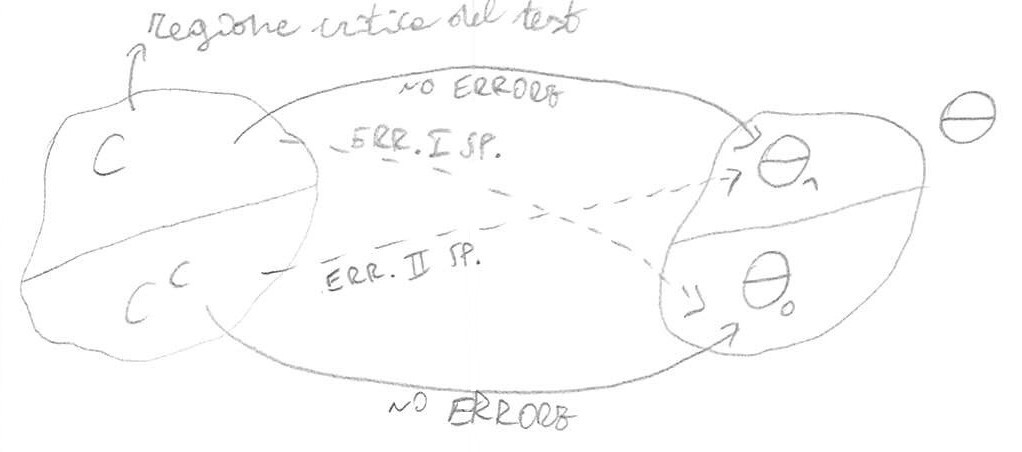
\includegraphics [width=12cm] {immagini/grafico_1.jpg}
\end{center}

\noindent \textbf{Esempio} Lancio di una moneta onesta. Consideriamo il campione casuale $(X_1,...,X_n)$ e il numero di teste $S_n = \sum_{i=1}^n X_i$. Vorremmo stimare la probabilità che esca testa con la media campionaria $\overline{X}_n$. In questo caso potremmo avere:
\\
$$\bigg \{
\begin{array}{rl}
H_0: & p=1/2 \\
H_1: & p \neq 1/2 \\
\end{array}
$$
\\
La regola di decisione consiste quindi nel rifiutare $H_0$ se $(X_1,...,X_n) \in C$ e invece rifiutare $H_0$ se $(X_1,...,X_n) \in C^c$. Ci piacerebbe trovare una regola di decisione che permetta di minimizzare la probabilità di commettere errori di I o II tipo. Purtroppo questo non è possibile, per la natura stessa della relazione che corre tra gli errori di I e II tipo. Di seguito un esempio che ci dà un'idea del perché:\\

\noindent \textbf{Esempio} Consideriamo un campione casuale $(X_1,...,X_n)$ da $N(\mu,\sigma^2)$ con $\sigma^2$ noto. Supponiamo che le nostre due ipotesi siano:
\\
$$\bigg \{
\begin{array}{lcr}
H_0: & \mu=\mu_0 & \text{ovvero } N(\mu=\mu_0,\sigma^2) \\
H_1: & \mu=\mu_1 & \text{ovvero } N(\mu=\mu_1,\sigma^2) \\
\end{array}
$$
con $\mu_1 > \mu_0$.\\
\\
\begin{center}
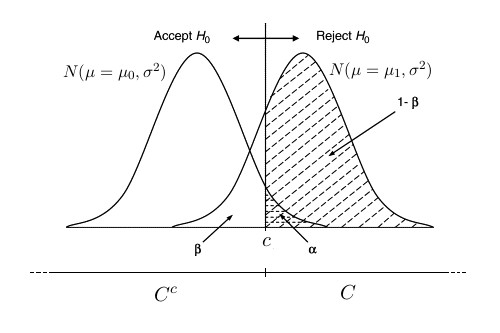
\includegraphics [width=12cm] {immagini/grafico_2.jpg}
\end{center}

Consideriamo $\alpha:= P(\text{rifiutare } H_0 \mid H_0 \text{ vera}) = P(\text{il nostro campione appartiene a C} \mid H_0 \text{ vera}) = P(\text{il nostro campione è } \leq c) = P(\text{commettere un errore di I tipo})$ e $\beta:= P(\text{non rifiutare } H_0 \mid H_0 \text{ falsa}) = P(\text{il nostro campione appartiene a } C^c \mid H_0 \text{ falsa}) = P(\text{il nostro campione è } \geq c) = P(\text{commettere un errore di II tipo})$. 
(Nota: $\alpha$ è detto \emph{livello di significatività del test})\\
È evidente che non è possibile annullare contemporaneamente sia $\alpha$ che $\beta$.\\
La procedura si divide quindi in due passi: il primo consiste nel \textbf{fissare} $\alpha$, il secondo nell'individuare la regola di decisione che minimizza $\beta$, in modo da trovare un test \textit{ottimo}.\\
\\
\\
%%%%LEZIONE 5 APRILE%%%%
Lezione del 05/04, ultima modifica 20/05, Andrea Gadotti
\\
In generale una statistica test si può descrivere come di seguito:\\
$$\bigg \{
\begin{array}{rl}
H_0: & \theta \in \Theta_0 \\
H_1: & \theta \in \Theta_1 \\
\end{array}
$$
\\
dove $\Theta$ è lo spazio dei possibili parametri della distribuzione e $\Theta = \Theta_0 \cup \Theta_1$.\\
Quello che vogliamo trovare è la regola di partizionamento che divida lo spazio dei campioni $C$ in $C_0$ e $C_1$ in funzione di $\alpha$ (deciso da noi). Per farlo imponiamo la condizione $\alpha = P(\underline{x} \in C \mid \theta \in \Theta_0)$. Vediamo ora un esempio con il lancio di una moneta:\\
\\
\noindent \textbf{Esempio} Consideriamo il campione casuale $(X_1,...,X_n)$ dove $X_i = 0$ con probabilità $p$ e $X_i = 1$ con probabilità $1-p$. Facciamo le nostre ipotesi:\\
$$\bigg \{
\begin{array}{rl}
H_0: & p \leq 1/2 \\
H_1: & p > 1/2 \\
\end{array}
$$
\\
Prediamo ora come regola di decisione $\frac{S}{n}=\frac{\sum X_i}{n}$. Deciso un $\alpha$ a nostra discrezione, imponiamo l'equazione in $k$:
$$ \alpha = P(S>k \mid p \leq 1/2) \; (= P(S>k \mid H_0 \text{ vera}))$$
A questo punto risolvendo l'equazione troveremo il $k$ per il quale rifiuteremo $H_0$ se $S>k$.\\
\\
\noindent \textbf{Esempio} Sia $(X_1,...,X_n)$ un campione casuale con $X_i \sim b(1,p)$ e sia\\
$$\bigg \{
\begin{array}{rl}
H_0: & p=p_0 \\
H_1: & p<p_0 \\
\end{array}
$$
\\
Sulla base dell'informazione circa $p$ contenuta in $(X_1,...,X_n)$ vogliamo sottoporre a verifica il sistema di ipotesi in questione. Procediamo in questo ordine:\\
\begin{enumerate}
\item [(a)] Prendiamo $S:=\sum X_i \sim b(n,p)$, che è di fatto il numero di successi. Sotto $H_0$ abbiamo che $S \sim b(n,p_0)$.
\item [(b)] Scegliamo una regola di decisione (usando anche la distribuzione -nota- di $S$ sotto $H_0$). Ovvero, individuiamo la \textit{regione di rifiuto del test}. A questo punto vorremo rifiutare $H_0$ a favore di $H_1$ quando $S \leq k$, dove $k$ è l'incognita che troveremo nel punto (c).
\item [(c)] Scelto il nostro $\alpha$, si ha che il valore di $k$ deve essere tale per cui 
			$$\alpha = P(S \leq k \mid p=p_0) = \displaystyle \sum_{s=0}^k \binom{n}{s} p_0^s (1-p_0)^{n-s}$$
A questo punto, essendo $\alpha$ fissato, abbiamo un'equazione in $k$ che risolta ci restituisce il suo valore.
\end{enumerate}
\textbf{Esempio particolare} Nella situazione generale sopra descritta prendiamo un caso particolare con $n=20$ e $p_0=0,7$. Decidiamo $\alpha = 0.15$. L'equazione diventa: $0,15 = \sum_{s=0}^k \binom{20}{s} 0,7^s 0,3^{20-s}$. Osserviamo che il valore di $P(S \leq k \mid p=0,7)$ per $k=11$ risulta $0,1133$, mentre per $k=12$ è $0,2277$. Quindi il nostro $k$ è compreso tra 11 e 12. In conclusione, se il nostro test dovesse presentare 12 (o più) successi, allora non rifiuteremmo $H_0$. In caso contrario scarteremmo $H_0$ a favore di $H_1$.

\begin{definizione} Sia $\beta := P(\underline{x} \in C_0 \mid \theta \in \Theta_1)$, ovvero $\beta$ è la probabilità (fissato $\alpha$) di commettere un errore di II specie. Chiamiamo \textit{potenza del test} il valore $\gamma := 1-\beta$. Un test risulta ottimale quando la sua potenza è massima. Notiamo che possiamo definire una \textit{funzione di potenza} $\gamma(t) := 1-\beta(t)$
\end{definizione}
\begin{oss} Prendendo di nuovo in considerazione l'esempio precedente sul campione casuale normale, è chiaro che una volta fissato $\alpha$, ovvero $c$, minore è $\mu_1$, più piccola è l'area sottesa dalla coda della relativa normale, ovvero $\beta$.
\end{oss}
\noindent \textbf{Esempio} Prendendo di nuovo in considerazione l'esempio precedente sulla bernoulliana, abbiamo che 
			$$\gamma(p) = P(S \leq k \mid p<p_0) = \displaystyle \sum_{s=0}^k \binom{n}{s} p^s (1-p)^{n-s}$$
Di seguito possiamo osservare il grafico della funzione:\\
\\
\begin{center}
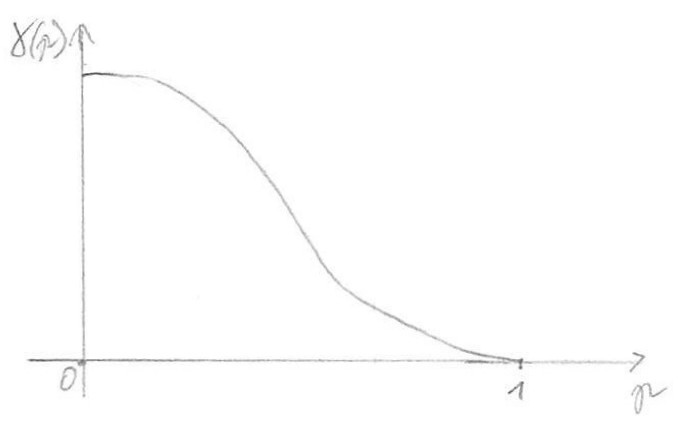
\includegraphics [width=12cm] {immagini/grafico_3.jpg}
\end{center}
\textbf{Osservazione} Il test in merito al precedente sistema di ipotesi relative a $p$ è un \textit{test esatto}, perché poggia sulla distribuzione \textit{esatta} di $S$ ($S \sim b(n,p)$). Questo però non accade sempre, e quindi talvolta è necessario ricorrere alla teoria asintotica e dei test approssimati.\\


\subsection{Esempi di statistiche test (generali e particolari)}

\textbf{Test per la media di una popolazione qualsiasi} Supponiamo di avere un campione casuale $(X_1,...,X_n)$ proveniente da una distribuzione \underline{non} nota di media $\mu$ e varianza $\sigma^2$ (finita) \underline{non} note.\\
Le nostre ipotesi sono 
$$\bigg \{
\begin{array}{rl}
H_0: & \mu=\mu_0 \\
H_1: & \mu>\mu_0 \\
\end{array}
$$
Decidiamo di ''condensare'' l'informazione presente nel campione circa $\mu$ e $\sigma^2$ tramite $\overline{X}_n$ e $S_n^2$ (che ricordiamo essere stimatori non distorti e consistenti), sapendo che $\overline{X}_n \stackrel{P}{\rightarrow} \mu$ e $S_n^2 \stackrel{P}{\rightarrow} \sigma^2$.\\
A questo punto, la nostra regola di decisione consisterà nel rifiutare $H_0$ a favore di $H_1$ se $\overline{X}_n$ è molto più grande di $\mu_0$.\\
Noi sappiamo che $\overline{X}_n \stackrel{a}{\sim} N \left( \mu, \frac{S_n^2}{n}\right)$, ovvero $\frac{\overline{X}_n-\mu}{S_n/\sqrt{n}} \stackrel{D}{\rightarrow} N(0,1) =: Z$\\
Usando questo risultato possiamo individuare la regione critica del test di livello $\alpha$ fissato. Imponiamo la seguente uguaglianza:

\begin{eqnarray}
\alpha 	&=& P(\overline{x} \in C \mid \mu=\mu_0) = P(\overline{X}_n \geq k \mid \mu=\mu_0) \nonumber \\
		&=& P \left( \frac{\overline{X}_n-\mu}{S_n/\sqrt{n}} \geq \frac{\overline{k}-\mu}{S_n/\sqrt{n}} \mid \mu=\mu_0 \right) \nonumber \\
		&=& P \left( \frac{\overline{X}_n-\mu_0}{S_n/\sqrt{n}} \geq \frac{\overline{k}-\mu_0}{S_n/\sqrt{n}} \right) = P(Z \geq z_{\alpha}) \nonumber
\end{eqnarray}

Dove $z_{\alpha}$ è il valore da cercare sulle tavole relative alla distribuzione normale in funzione dell'$\alpha$ scelto. Nota: l'ultima uguaglianza è in realtà un'approssimazione che è tanto più corretta quanto più grande è $n$.\\
In definitiva, abbiamo che $C = \lbrace \underline{x} \in \varkappa \; : \; \frac{\overline{X}_n-\mu_0}{S_n/\sqrt{n}} \geq z_{\alpha} \rbrace = \lbrace \underline{x} \in \varkappa \; : \; \overline{X}_n \geq \mu_0 + z_{\alpha} \frac{S}{\sqrt{n}} \rbrace$\\

Possiamo anche considerare la \textit{funzione di potenza approssimata}:

\begin{eqnarray}
\gamma(\mu) = 1- \beta(\mu) 	&=& P(\overline{X}_n \geq \mu_0 + z_{\alpha} \sigma / \sqrt{n} \mid \mu > \mu_0) \nonumber \\
							&=& P \left(\frac{\overline{X}_n-\mu}{\sigma / \sqrt{n}} \geq \frac{\mu_0 + z_{\alpha} \sigma / \sqrt{n} - \mu}{\sigma / \sqrt{n}} \right) \nonumber \\
							&=& 1-P \left( Z \geq z_{\alpha} + \frac{\sqrt{n}(\mu_0 - \mu)}{\sigma} \right) \nonumber \\
							&=& 1-\Phi \left( z_{\alpha} + \frac{\sqrt{n}(\mu_0 - \mu)}{\sigma} \right) \nonumber
\end{eqnarray}

dove $\Phi$ è la funzione di ripartizione di $N(0,1)$.\\
Notiamo che il valore di $\gamma(\mu)$ tende a 1 per $n \rightarrow \infty$. Intuitivamente, questo è esattamente ciò che ci aspettiamo, in quanto più è grande $\mu$, più esso è distante dal nostro $\mu_0$, e di conseguenza è lecito aspettarsi che la probabilità che un campione abbia media vicina a $\mu$ sarà bassa, ovvero la potenza del test è elevata.\\
È chiaro quindi che una funzione di potenza è tanto migliore quanto più il suo grafico sta vicino alla retta $y=1$.\\
\\
\textbf{Esempio} In riferimento al caso generale appena trattato, supponiamo di avere $\mu_0=12$, $\overline{X}_n=14,3$, $S_n^2=22,5$, $n=50$. Se fissiamo $\alpha=0,05$, usando le tavole per la distribuzione normale $N(0,1)$ troviamo $z_{\alpha}=1,645$. Ne segue che $k=12+1,645\sqrt{22,5/50}$, che è minore di $14,3$. Concludiamo quindi rifiutando $H_0$.\\
\\
\textbf{Esempio di test esatto con t di Student} Abbiamo $(X_1,...,X_n)$ campione casuale da $N(\mu,\sigma^2)$ con $\mu$ e $\sigma^2$ non noti. Le nostre ipotesi sono:
$$\bigg \{
\begin{array}{rl}
H_0: & \mu=\mu_0 \\
H_1: & \mu>\mu_0 \\
\end{array}
$$
Sappiamo che $\overline{X}_n \stackrel{H_0}{\sim} N(\mu_0,\sigma^2/n)$ e quindi:
$$T:= \frac{\overline{X}_n - \mu_0}{S_n / \sqrt{n}} = \frac{\overline{X}_n - \mu_0}{\sigma / \sqrt{n}} \frac{1}{\sqrt{S_n^2 / \sigma^2}} \sim \frac{Z}{S_n / \sqrt{n}} \sim t_{n-1}$$
(vedi pag. 17 e pag. 12)\\
A questo punto, possiamo trovare il nostro valore critico $k$ usando le tavole della distribuzione $t_{n-1}$.\\
Notiamo che quello appena mostrato è un \textit{test esatto}, in quanto non si basa su un'approssimazione dello stimatore per valori elevati di $n$ (usando ad esempio il TLC), bensì usa la sua distribuzione reale (in questo caso la distribuzione $t_{n-1}$).
\\ \\
Lezione 08/04, ultima modifica 20/05, Michele Nardin
\\ \\
\noindent \textbf{Esempio di test bilaterale}
Sia $(X_1,...,X_n)$ un campione casuale da una distribuzione avente media $\mu$ e varianza $\sigma^2$ finite. 
Considerato il fatto che non abbiamo informazioni sulla distribuzione delle variabili casuali, 
ci appoggeremo su di un test \textit{approssimato}.
Supponiamo di voler verificare la seguente ipotesi relativa alla media della distribuzione:

$$\bigg \{
\begin{array}{rl}
H_0: & \mu = \mu_0 \\
H_1: & \mu \neq \mu_0 \\
\end{array}
$$
\\ \\
Seguendo la falsariga di quanto visto sopra, procediamo come segue:

\begin{enumerate}
\item [(a)] Prendiamo $\overline{X}=\displaystyle \frac{\sum X_i}{n}$, che è stimatore della media del campione. Non conoscendo la distribuzione esatta delle variabili, consideriamo la distribuzione approssimata: sotto $H_0$ abbiamo che $\overline{X} \stackrel{a}{\sim} N(\mu_0,\sigma^2 / n) $ (questo, come già detto varie volte, per il TLC).

\item [(b)] Scegliamo una regola di decisione: usando anche la distribuzione asintotica di $\overline{X}$ sotto $H_0$, individuiamo la \textit{regione di rifiuto del test}. 
Dobbiamo trovare quindi due valori $h,k \in \mathbb{R}$ 
tali per cui \textit{rifiuto} $H_0$ se $\overline{X_n} \leq h$ o $\overline{X_n} \geq k$.

\item [(c)] Scelto il livello di confidenza $\alpha$, si ha che $h,k$ vanno scelti in modo tale per cui 
$$\alpha = P(\overline{X} \leq h \vee \overline{X} \geq k \mid \mu=\mu_0)$$
Grazie alla normalità della distribuzione asintotica, possiamo supporre che la distribuzione di $\overline{X_n}$ sia simmetrica, per lo meno da un certo $n$ in poi (ricordiamo che, per campioni con numerosità superiori a 30, l'approssimazione è già buona).

Questo ci permette di scrivere
$$\frac{\alpha}{2} = P(\overline{X} \leq h \mid \mu=\mu_0) = P(\overline{X} \geq k \mid \mu=\mu_0)$$

Dato che $$\frac{\overline{X} - \mu_0}{S_n / \sqrt{n}} \stackrel{D}{\to} N(0,1)$$
denotato con $z_{\alpha/2}$ il quantile di ordine $\alpha / 2$ della normale standard, la regione critica (di rifiuto) sarà
$$C=\left\{ \underline{x}=(x_1,...,x_n) \in X : \left| \frac{\overline{X} - \mu_0}{S_n / \sqrt{n}} \right| \geq z_{\alpha/2} \right\}$$
da cui $$k =  \frac{S_n}{\sqrt{n}}z_{\alpha/2} + \mu_0 (= -h )$$
\end{enumerate}

Consideriamo inoltre la funzione di potenza associata, sempre sfruttando l'approssimazione normale ed il fatto che, per n grande, $S_n \approx \sigma$:

\begin{align*}
\gamma(\mu) &=P(\overline{X} \leq \mu_0 - \frac{S_n}{\sqrt{n}}z_{\alpha/2} \mid \mu \neq \mu_0 ) 
+ P(\overline{X} \geq \mu_0 + \frac{S_n}{\sqrt{n}}z_{\alpha/2} \mid \mu \neq \mu_0 )
\\ & \approx \Phi\left( \frac{\sqrt{n}(\mu_0 - \mu)}{\sigma} - z_{\alpha / 2} \right)
 + \left[ 1 - \Phi\left( \frac{\sqrt{n}(\mu_0 - \mu)}{\sigma} - z_{\alpha / 2} \right) \right]
\end{align*}
Di seguito possiamo osservare il grafico della funzione:\\
\begin{center}
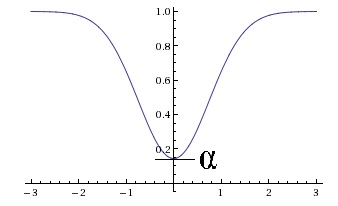
\includegraphics {immagini/potenza_bilaterale.jpg}
\end{center}

\textbf{Osservazione:} i test costruiti usando t di Student sono più conservativi rispetto a quelli costruiti con approssimazione Normale, nel senso che è più facile che un test venga accettato usando la prima rispetto alla seconda. Questo è dato dal fatto che la distribuzione t di student ha le code più pesanti rispetto alla normale! (in particolare fissato un 
$\alpha \in (0,1)$,
 i quantili della normale standard $z_{\alpha/2}$ sono più piccoli dei quantili della t di Student con $n-1$ gradi di libertà $t_{\alpha/2; n-1}$, cioè 
$|z_{\alpha/2}| < |t_{\alpha/2; n-1}|$)
\\ \\

%%%%LEZIONE 12 APRILE%%%%
Lezione del 12/04, ultima modifica 20/05, Andrea Gadotti\\
\\
\\

\textbf{Esempio di test t-Student per due campioni}\\
Campione $(X_1,...,X_{n_1})$ da $N(\mu_1,\sigma^2)$ e $(Y_1,...,Y_{n_2})$ da $N(\mu_2,\sigma^2)$ indipendenti. La varianza $\sigma$ è la stessa ma non è nota.\\
Supponiamo di avere elementi per pensare che:
$$\bigg \{
\begin{array}{rl}
H_0: & \mu_1=\mu_2 \\
H_1: & \mu_1>\mu_2 \\
\end{array}
$$
Abbiamo che $\overline{X}_1 - \overline{X}_2 \sim N(\mu_1 - \mu_2, \sigma_1/n_1 + \sigma_2/n_2)$.\\
Prendiamo ora 
$$S_p^2:= \frac{(n_1-1)S_1^2 + (n_2-1)S_2^2}{n-2}$$ 
dove $n=n_1+n_2$.\\
Abbiamo che:
$$T:= \frac{(\overline{X}_1 - \overline{X}_2)-(\mu_1-\mu_2)}{S_p \sqrt{1/n_1+1/n_2}} \; \stackrel{H_0}{\sim} \; t_{n-2}$$
dove abbiamo usato anche il fatto che $S_p^2$ è una chi-quadro con $n-2$ gradi di libertà (vedi pag. 19).\\
In conclusione, avremo che la nostra regione critica sarà $C=\lbrace (\underline{x},\underline{y}) \mid T \geq t_{n-2;\alpha} \rbrace$.\\
\\
\textbf{Esempio con bernoulliana} Abbiamo $(X_1,...,X_n)$ campione casuale da $b(1,p)$ (ricordiamo: media $p$, varianza $p(1-p)$). Le nostre ipotesi sono:
$$\bigg \{
\begin{array}{rl}
H_0: & p=p_0 \\
H_1: & p=p_1 \\
\end{array}
$$
con $p_1<p_0$. Consideriamo
$$\hat{p}_n := \frac{\sum X_i}{n} \stackrel{a}{\sim} N \left( p, \frac{p(1-p)}{n} \right)$$
Abbiamo quindi:
$$Z:= \frac{\hat{p}_n-p_0}{\sqrt{\frac{\hat{p}_n (1-\hat{p}_n)}{n}}}$$
A questo punto imponiamo: $\alpha = P(Z \leq z_{\alpha} \mid H_0)$.\\
\\
\textbf{Esempio di test sulla varianza} Campione casuale $(X_1,...,X_n)$ da $N(\mu,\sigma^2)$, $\mu$ e $\sigma^2$ non noti. Le nostre ipotesi sono: 
$$\bigg \{
\begin{array}{rl}
H_0: & \sigma^2=\sigma_0^2 \\
H_1: & \sigma^2=\sigma_1^2 \\
\end{array}
$$
con $\sigma_1^2 > \sigma_0^2$.
Notiamo che $\frac{n-1}{\sigma_0^2} S_n^2 \stackrel{H_0}{\sim} \chi_{n-1}^2 =: W$. (Nota: come in molti esempi precedenti, il fatto che sia "intelligente" tirare fuori queste osservazioni che portano all'analisi di distribuzioni conosciute è "calato dall'alto", almeno per ora).\\
Imponiamo:
$$\alpha = P \left( \frac{n-1}{\sigma^2} S_n^2 \mid \sigma^2=\sigma_0^2 \right) = P \left( \frac{n-1}{\sigma_0^2} S_n^2 \right)$$
Quindi $k=w_{\alpha;n-1}$. In conclusione, rifiuto $H_0$ se $W \geq w_{\alpha;n-1}$.\\
\textbf{Esempio} In riferimento al caso generale appena trattato, supponiamo di avere $n=25$, $\sigma_0^2=15$, $\sigma_1^2=20$, $s_n^2=17,4$ e $\alpha=0,05$. Allora:
$$k=w_{0,05;(25-1)} = w_{0,05;24} = 36,415 > 27,84 = \frac{25-1}{15} 17,4 = \frac{n-1}{\sigma_0^2} s_n^2 = w$$
In conclusione, non rifiutiamo $H_0$.\\
\\
\textbf{Esempio con due campioni normali} Campione $(X_1,...,X_{n_1})$ da $N(\mu_1,\sigma_1^2)$ e $(Y_1,...,Y_{n_2})$ da $N(\mu_2,\sigma_2^2)$ indipendenti. $\mu_i$ e $\sigma_i^2$ non noti. Le nostre ipotesi sono:
$$\bigg \{
\begin{array}{rl}
H_0: & \sigma_1^2=\sigma_2^2 \\
H_1: & \sigma_1^2 \neq \sigma_2^2 \\
\end{array}
$$
Nota: l'ipotesi dell'uguaglianza delle due varianze prende il nome di omoschedasticità.\\
Sappiamo che $S_i^2 \stackrel{P}{\rightarrow} \sigma_i^2$. Inoltre
$$W:= \frac{S_2^2 / \sigma_2^2}{S_1^2 / \sigma_1^2} = 
\frac{\frac{(n_2-1) S_2^2}{\sigma_2^2} \frac{1}{n_2-1}} {\frac{(n_1-1) S_1^2}{\sigma_1^2} \frac{1}{n_1-1}} 
\sim F_{(n_2-1),(n_1-1)}$$
(vedi pag. 20)\\
Sotto $H_0$ abbiamo chiaramente che $W:= \frac{S_2^2 / \sigma_2^2}{S_1^2 / \sigma_1^2} = \frac{S_2^2}{S_1^2}$. La nostra regola di decisione consisterà nel rifiutare $H_0$ a favore di $H_1$ se $\frac{S_2^2}{S_1^2}$ è ''lontano'' da 1, ovvero se $W<k_1$ o $W>k_2$, dove $k_1$ e $k_2$ dipendono dalla distribuzione di $W= \frac{S_2^2}{S_1^2}$ e dal valore di $\alpha$. Perciò, dividendo equamente in due parti la probabilità di errore, le due equazioni risultano:
$$\alpha/2 = P(W>k_2 \mid \sigma_1^2=\sigma_2^2) \; \; \text{ e } \; \; 1-\alpha/2 = P(W<k_1 \mid \sigma_1^2=\sigma_2^2)$$
In conclusione, 
$$C= \lbrace (\underline{x_1},\underline{x_2}) \; : \; \frac{S_2^2}{S_1^2} < w_{(n_2-1),(n_1-1);\alpha/2} \; \; \text{ o } \; \; \frac{S_2^2}{S_1^2} > w_{(n_2-1),(n_1-1);1-\alpha/2}$$
In riferimento al caso generale appena trattato, supponiamo di avere $n_1=14$, $n_2=10$ $s_1^2=17,4$, $\sigma_1^2=20$, $s_2^2=37,9$ e $\alpha=0,05$.\\
Come nel caso generale, diciamo $W:=S_2^2/S_1^2 \sim F_{(n_2-1),(n_1-1)}$.\\
Abbiamo che $w_{(10-1),(14-1);0,025}=3,31$ e $w_{(10-1),(14-1);0,975}=1/w_{13,19;0,025}=1/3,76=0,26$.\\
Poiché $s_2^2/s_1^2=37,9/17,4=2,178$, decidiamo di non rifiutare $H_0$.
\chapter{Seconda parte del corso}
Lezioni dal 15/04 al 06/05 comprese. Autore: Marco Peruzzetto.\\
Questa parte comprende ed amplia le cose viste a lezione, estendendo alcune dimostrazioni e osservazioni. Quanto non fatto in classe verrà denotato da un (*).\\
\\
\textbf{Definizione:} Sia $\vec{X}\coloneqq (X_1,\ldots X_n)$ un vettore casuale da distribuzione $F(\vec{x}, \theta)$ per $\theta\in \Theta$ e sia $f_{X_i}(x_i,\theta)$ la corrispondente funzione densità di ciascuna $X_i$, $\forall 1\leq i\leq n$. Indicheremo con $\vec{x}=(x_1,\ldots,x_n)$ una qualsiasi possibile determinazione del vettore $\vec{X}$. Essa conterrà tutta l'informazione in merito a $\theta$. Possiamo allora definire la \textit{Funzione di Verosimiglianza} come la funzione:
$$L\left(\theta, \vec{x}\right)\coloneqq f_{\vec{X}}(\vec{x},\theta)=f_{(X_1,\ldots,X_n)}(x_i,\ldots,x_n,\theta)\mbox{ , } \theta\in \Theta, $$ che rappresenta quindi la funzione di densità dell'intero vettore in dipendenza del parametro $\theta$. Nel caso in cui il vettore casuale sia un campione casuale, allora tutte le variabili casuali di cui esso è composto saranno i.i.d., ragion per cui la funzione di massima verosimiglianza assumerà la seguente tipica forma:
$$L\left(\theta, \vec{x}\right)=\prod_{i=1}^n f_{X_i}\left(x_i, \theta\right) \mbox{ , } \theta\in \Theta.$$
Esiste anche la \textit{Funzione di Log-Verosimiglianza} definita come $l(\theta,\vec{x})\coloneqq \log\big(L(\theta, \vec{x})\big)$. 
\\ 
\\
\textit{Esempio:} Sia $(X_1,\ldots,X_n)\sim Poisson(\theta)$. Allora $$L(\theta, \vec{x})=\prod_{i=1}^n \frac{e^{-\theta}\theta^{x_i}}{x_i !}\mathbbm{1}_{\mathbb{N}}(x_i)=\frac{e^{-n\theta}\theta^{\sum_{i=1}^n x_1}}{\prod_{i=1}^n x_i !}\prod_{i=1}^n \mathbbm{1}_{\mathbb{N}}(x_i)$$ da cui $$l(\theta, \vec{x})=\log(\theta)\sum_{i=1}^n x_i   -n\theta - \sum_{i=1}^n \log(x_i !).$$ 
\\ \\
\textit{Osservazioni:} \begin{itemize}

\item La funzione di verosimiglianza dà un valore alla probabilità che $\vec{x}$ provenga da $F_{\vec{X}}(\vec{x},\theta)$ per tutti i differenti valori di $\theta\in \Theta$.

%\item L'approccio della verosimiglianza al problema della stima produce automaticamente un candidato stimatore. Infatti essa rappresenta una quantità numerica che esprime l'ordine di preferenza circa $\theta$ sulla base dell'informazione contenuta in $\vec{x}$.

\item Nella funzione di verosimiglianza è stato volontariamente invertito il parametro $\theta$ con il parametro $\vec{x}$ rispetto, ad esempio, alla funzione densità. La ragione si basa sulla diversa interpretazione della stessa: a tutti gli effetti la funzione di verosimiglianza non è altro che la funzione densità del vettore casuale $\vec{X}$. Quindi essa può essere vista in due modi diversi: il primo interpreta la funzione $L$ come una funzione di $\vec{x}$, e quindi del risultato, una volta fissato il valore del parametro (perciò $L$ esattamente la densità), mentre il secondo la interpreta come una funzione del parametro $\theta$, per un fissato valore del risultato $\vec{x}$. Proprio in quest'ultimo caso ha senso parlare di verosimiglianza: il valore assunto da $L$ indica quanto verosimilmente il valore di un parametro $(\theta)$ sia corretto rispetto al risultato che si possiede $(\vec{x})$. 

\item (*) Data una determinazione $\vec{x}$ di $\vec{X}$, la funzione $L(\cdot, \vec{x})$, essendo la densità del vettore casuale, esprime la probabilità che $\vec{X}$ assuma proprio il valore $\vec{x}$. Ciò avviene in modo diretto se le variabili componenti il vettore sono discrete e tramite integrazione se continue. Ha senso allora chiedersi, data una determinazione $\vec{x}_0$ di $\vec{X}$, quale sia (se esiste) un possibile valore $\theta_0\in \Theta$ capace di massimizzare il valore di $L(\theta_0,\vec{x}_0)$. Massimizzare tale valore significa infatti per quanto detto, andare a massimizzare la probabilità che $\vec{X}$ assuma il valore $\vec{x}_0$. Ciò avverrà direttamente se il vettore casuale è discreto, ma anche se è continuo, e ciò banalmente grazie alla monotonia dell'integrale, in quanto, se riusciamo a massimizzare la funzione con $\theta$ anche l'integrale (ovviamente integrando in $d\vec{x}$) sarà massimo (rivedere).

\item L'importanza di cercare il valore del parametro che massimizzi $L$ fissata la determinazione risiede nel fatto che spesso in statistica si ha a che fare con poche determinazioni e si parte dunque dall'evidente presupposto che se il campionamento effettuato ci ha fornito quelle specifiche determinazioni, esse debbano essere mediamente le più probabili. Tale presupposto viene in effetti denominato \textit{Principio di ``Rational Belief''}. La probabilità che dato quel campione casuale si ottengano quelle determinazioni la immagineremo quindi come la massima possibile. Cercheremo dunque un $\theta\in \Theta$ che soddisfi a ciò. È inevitabile che attraverso la verosimiglianza si possano ottenere degli stimatori del parametro.

\item La funzione di $\log$-verosimiglianza è stata introdotta pressoché per il semplice motivo di semplificare i calcoli quando si cerca di andare a massimizzare la funzione di verosimiglianza. Essa risulta dunque essere comoda, in quanto, essendo il logaritmo una funzione strettamente crescente, il massimizzante di $l(\cdot,\cdot)$ coinciderà con quello di $L(\cdot,\cdot)$.
\end{itemize}
\textit{Esempio} (Problema dei Pesci): Dato un lago, lo scopo è cercare di stimare la grandezza $N$ della popolazione dei pesci che vi vivono. Un modo può essere il seguente: si pescano esattamente $N_1$ pesci, i quali vengono in qualche modo marcati. In seguito, dopo aver permesso un mescolamento, si esegue un'ulteriore pesca, di $n$ pesci. Si nota che fra questi ve ne sono $n_1$ marcati. Vogliamo capire quale sia il valore di $N$ più plausibile. Nel nostro caso avremo un vettore casuale composto da una sola variabile, ovvero $\vec{X}=(X)$, la quale ha valori in $\mathbb{N}$ (ed è quindi discreta) e restituisce i possibili valori di $n_1$. La sua densità sarà allora fornita in modo diretto e coincide con la funzione di verosimiglianza in quanto vi è una singola variabile casuale nel vettore. L'insieme dei parametri sarà anch'esso $\mathbb{N}$. Chiaramente vogliamo stimare il più plausibile valore di $\theta=N$. Avremo dunque: 
$L(N)\coloneqq L(N,n_1)=\mathbb{P}[X=n_1]=\frac{\binom{N}{n_1}\binom{N-N_1}{n-n_1}}{\binom{N}{n}}.$ Per effettuare un esempio concreto: con $N_1=300$ e $n=80$, se la nostra determinazione ottenuta fosse $n_1=30$, allora il parametro che massimizza la probabilità sarebbe $N\sim 1200$. È quindi plausibile che nel lago viva una quantità di pesci che si aggira effettivamente intorno ai 1200 esemplari.
\\  \\
\textbf{Definizione:} Assumiamo che la funzione di verosimiglianza sia dervabile per il parametro $\theta$. Allora la funzione $S(\theta)\coloneqq \frac{\partial}{\partial \theta}\l(\theta, \vec{x})$ viene detta \textit{Score Function}. L'equazione $S(\theta)=0$ è chiamata \textit{Equazione di Stima}. 
\\
\\
\textit{Osservazione:} Osserviamo che poiché la funzione densità di una qualsiasi variabile casuale è sempre positiva o nulla, in quanto prodotto, lo dovrà essere anche la parte di $L(\cdot,\cdot)$ che non dipende da $\theta$. Ne segue che, se vogliamo massimizzare la funzione di verosimiglianza, possiamo direttamente limitarci a considerare solo i valori di $\theta\in \Theta$ che rendano $L(\cdot,\cdot)$ strettamente positiva per ciascuna determinazione $\vec{x}$ fissata o scelta. Dunque si può restringere senza perdere generalità l'insieme $\Theta$ in modo da avere valori che non permettono a $L(\cdot,\cdot)$ di annullarsi. $S(\theta)$ risulta quindi avere una buona definizione, in quanto non è necessario effettuare ulteriori ipotesi su $l(\cdot,\cdot)$, essendo:  
$$S(\theta)=\frac{\partial}{\partial\theta}l(\theta,\vec{x})=\frac{\partial}{\partial\theta}\log\big(L(\theta,\vec{x})\big)=\frac{1}{L(\theta,\vec{x})}\frac{\partial}{\partial\theta}L(\theta,\vec{x}).$$
\textbf{Definizione:} La funzione di verosimiglianza induce uno stimatore del parametro $\theta$. Esso sarà chiamato \textit{Stimatore di Massima Verosimiglianza} ed è così definito: $\hat{\theta}_n=\hat{\theta}_n(\vec{X})\coloneqq \ar\big\{\max_{\theta\in \Theta}\{L(\theta,\vec{X})\}\big\}=\ar\big\{\max_{\theta\in \Theta}\{l(\theta,\vec{X})\}\big\}$.
\\
\\
\textit{Osservazioni:}
\begin{itemize}
\item Da ora in poi l'argomento delle funzioni $L(\cdot,\cdot)$ e $l(\cdot,\cdot)$ verrà interpretato a seconda della convenienza e del senso sia come $(\theta,\vec{x})$, ovvero come determinazione, oppure come $(\theta, \vec{X})$, ovvero vettore casuale. Osserviamo che in quest'ultimo caso, le funzioni $L$ e $l$ diventano esse stesse automaticamente variabili casuali o stimatori, che dir si voglia. Ciò si ripercuote inevitabilmente sulle funzioni ad esse collegate, ad esempio su $S(\theta)$.
\item Se $L(\cdot,\cdot)$ o $l(\cdot,\cdot)$ sono derivabili rispetto a $\theta$, la funzione indipendente da $\theta$ che risolve $\forall \vec{x}$ l'equazione di stima $S(\theta)=0$ fornisce effettivamente lo stimatore di massima verosimiglianza. Oppure, equivalentemente, potremmo dire che lo stimatore di massima verosimiglianza $\hat{\theta}_n(\vec{X})$ è quello che soddisfa l'equazione $S\big(\hat{\theta}_n(\vec{X})\big)=0$.
\item In generale non vi è garanzia che lo stimatore di massima verosimiglianza esista, oppure, se esiste, che esso sia unico. Tuttavia nel caso di famiglie di densità che rispettino certe ipotesi di regolarità (per esempio le famiglie esponenziali) tale problema non si pone.
\item Anche assumendo che tale stimatore esista e sia unico, non è detto che sia sempre ottenibile analiticamente. Talvolta sarà necessario ricorrere a metodi numerici per la risoluzione dell'equazione di stima.
\end{itemize}
\textit{Esempi:}
\begin{enumerate}
\item Riprendiamo l'esempio precedente ove avevamo il campione casuale con variabili distribuite come poissoniane di parametro $\theta$. 
La funzione di log-verosimiglianza era data da $$l(\theta, \vec{x})=\log(\theta)\sum_{i=1}^n x_i   -n\theta - \sum_{i=1}^n \log(x_i !)$$
sicché otteniamo subito che $$S(\theta)=\frac{1}{\theta}\sum_{i=1}^n x_i   -n$$
Si deduce allora immediatamente l'equazione di stima $\frac{1}{\theta}\sum_{i=1}^n x_i   -n=0 \Rightarrow \theta=\frac{1}{n}\sum_{i=1}^n x_i$
Ma allora $$\hat{\theta}_n(\vec{X})=\overline{X}_n=\frac{1}{n}\sum_{i=1}^n X_i$$ che è la media campionaria.\\
\\
\item Sia $\vec{X}\coloneqq (X_1,\ldots,X_n)\sim U[(0,\theta)]$. 
Allora $$f_X(x,\theta)\coloneqq \frac{1}{\theta}\mathbbm{1}_{[0,\theta]}(x)$$ 
Perciò $$L(\theta, \vec{x})=\frac{1}{\theta^n}\prod_{i=1}^n\mathbbm{1}_{[0,\theta]}(x_i)=\frac{1}{\theta^n}\mathbbm{1}_{[X_{(n)},+\infty]}(\theta)\Rightarrow \hat{\theta}_n(\vec{X})=X_{(n)}.$$\\
\\
\item Sia $\vec{X}\coloneqq (X_1,\ldots,X_n)\sim \exp(\beta)$, $\beta>0$. 
Allora $f_X(x,\theta)\coloneqq \beta e^{-\beta x}\mathbbm{1}_{\mathbb{R}_+}(x)$. 
Perciò $$L(\theta, \vec{x})=\big(\beta^n e^{-\beta\sum_{i=1}^n x_i}\big)\mathbbm{1}_{\mathbb{R}_+^n}(\vec{x})\Rightarrow l(\theta, \vec{x})=n\log(\beta)-\beta\sum_{i=1}^n x_i$$ 
Otterremo allora l'equazione di stima $0=S(\beta)=n\beta-\sum_{i=1}^n x_i$, da cui subito si deduce che anche in questo caso $\hat{\theta}_n=\overline{X}_n$.\\
\\
\item \textit{(Troncamento)} Sia sempre $\vec{X}\coloneqq (X_1,\ldots,X_n)\sim \exp(\beta)$. Naturalmente ciascuna variabile casuale ha come codominio i reali non negativi. Possiamo supporre di aver effettuato gli $n$ rilevamenti dal campione casuale e di essere riusciti a individuarne esattamente $m$ puntualmente (che senza perdita di generalità immagineremo essere i primi $m$), mentre dei restanti $n-m$ immaginiamo di aver rilevato solamente che il loro valore supera una certa soglia fissta $T>0$. Il campione contiene quindi due tipi di informazione da coniugare nella funzione di massima verosimiglianza, che avrà stavolta una forma un po' diversa. La indicheremo con $L'$. Otteniamo: \\ 

\begin{eqnarray*}
L'(\beta,\vec{x}) &=&\prod_{i=1}^m f_{X_i}(x_i,\beta)\cdot\prod_{i=m+1}^n \mathbb{P}[X_i>T] \\
&=& \prod_{i=1}^m f_{X_i}(x_i,\beta)\cdot\prod_{i=m+1}^n \left(1-F_{X_i}(T,\beta)\right) \\
&=& \prod_{i=1}^m \beta e^{-\beta x_i} \cdot\prod_{i=m+1}^n \int_T^{+\infty} \beta e^{-\beta x_i}dx_i \\
&=& \beta^m e^{-\beta \sum_{i=1}^m x_i} \cdot e^{-\beta (n-m)T}
\end{eqnarray*}

Da cui $$l'(\beta,\vec{x})\coloneqq \log\left(L'(\beta,\vec{x})\right)=m\log(\beta)-\beta\sum_{i=1}^m x_i -\beta (n-m)T.$$ 
Inoltre possiamo definire anche qui una score function nel modo naturale: $$S'(\beta)\coloneqq \frac{\partial}{\partial\beta}l'(\beta,\vec{x})$$ da cui, uguagliando a 0 si può ottenere l'equazione di stima $$\frac{m}{\beta}-\sum_{i=1}^m x_i-(n-m)T=0$$ 
Si deduce così lo stimatore di massima verosimiglianza con troncamento a $T$, dato da $$\hat{\beta}_n'(\vec{X})=\frac{\sum_{i=1}^m X_i +(n-m)T}{m}.$$
\end{enumerate}

\section{Efficienza}
Dato uno stimatore $T_n$ di un campione casuale $\vec{X}\coloneqq (X_1,\ldots,X_n)$ possiamo partire dal concetto di errore quadratico medio $\mse_\theta(T_n)=\var_\theta(T_n)+B_\theta^2(T_n)$. Lo scopo sarà quello di cercare stimatori che minimizzino il più possibile tale valore. Il problema presenta alcune difficoltà: per fare un piccolo esempio, sia $\theta_0\in \Theta$ e consideriamo il seguente stimatore banale $U_n(\vec{X})\coloneqq \theta_0$. È ora evidente che se da una parte $\mse_{\theta_0}(U_n)=0$, sicché nessun altro stimatore può essere uniformemente migliore di $U_n$, dall'altra appare chiaro che di un siffatto stimatore non ci si possa attendere molto, e nemmeno fidare, in quanto esso ignora completamente tutta l'informazione contenuta nel vettore casuale. La difficoltà di trovare stimatori che abbiano errore quadratico medio minimo è dunque legata a due aspetti principali: spesso la struttura di $\mse$ è complicata in quanto contiene aspetti legati al parametro $\theta$; inoltre la classe degli stimatori competitori di $\theta$ è quasi sempre troppo ampia. \\ Cercheremo allora di semplificare il problema restringendo un po' il campo: considereremo solo gli stimatori non distorti, per andare poi a cercare tra questi quelli con varianza minima.  
\\
\\
\textit{Esempio:} Sia $\vec{X}\coloneqq (X_1,\ldots,X_n)\sim Poisson(\lambda)$. In tal caso si verifica subito che $\mathbb{E}[X]=\var[X]=\lambda$. Ne segue che sia lo stimatore media campionaria $\overline{X}_n$ sia lo stimatore varianza campionaria $S_n^2$ sono due stimatori non distorti di $\lambda$. Si ha tuttavia che $\var[\overline{X}_n]=\frac{\lambda}{n}\leq\frac{\lambda}{n}\left(1+\frac{2n\lambda}{n-1}\right)=\var[S_n^2]$. Preferiremo dunque la media campionaria. Ma consideriamo ora il seguente stimatore così definito, per $a\in [0,1]$ fissato, $W_{n,a}(\vec{X})\coloneqq a\overline{X}_n +(1-a)S_n^2$. Anch'esso è non distorto. Sorgono così due difficoltà da affrontare: ammesso che $\overline{X}_n$ sia migliore (i.e. con varianza più piccola) di $S_n^2$, esso è anche migliore di ogni stimatore $W_{n,a} \forall a$ oppure esso è il migliore tra tutti gli stimatori non distorti di $\lambda$? Esiste un limite inferiore alla varianza? Se infatti esso esistesse, darebbe operatività alla scelta dello stimatore, in quanto se trovassimo uno stimatore che raggiunge tale limite, sapremo che non è necessario cercare ulteriormente per migliorare le nostre possibilità. Ebbene, tale limite esiste sicuramente, sotto alcune ulteriori ipotesi di regolarità da addure alla non distorsione per gli stimatori.
\\
\\
\textbf{Definizione:} Una \textit{Famiglia Regolare} è una famiglia di densità che soddisfa le seguenti condizioni di regolarità:
\begin{enumerate}[noitemsep]
\item \textit{Condizione di Indentificabilità:} i valori delle densità sono distinti al variare del parametro, ovvero $\theta\neq \theta' \Longrightarrow f_X(x,\theta)\neq f_X(x,\theta')$.
\item Le funzioni densità hanno supporto comune $\forall \theta\in\Theta$ e il loro supporto non dipende in alcun modo dal parametro $\theta$.
\item Le funzioni sono di classe $C^2$ rispetto alla variabile $\theta$
\item Rispetto a $\theta$, è lecito lo scambio tra le derivate e l'integrale.
\end{enumerate}
\textbf{Definizione:} Sia $\vec{X}=(X_1,\ldots, X_n)$ un campione casuale. Allora la funzione
\begin{align*}
I:\Theta &\longrightarrow  \mathbb{R} \\
I(\theta)  &\coloneqq   \mathbb{E}_\theta[S(\theta)^2]=\mathbb{E}_\theta\Bigg[\left(\frac{\partial}{\partial \theta}l(\theta,\vec{X})\right)^2\Bigg]
\end{align*}
viene denominata \textit{Informazione di Fisher} del campione casuale.
\\
\\
\textit{Osservazioni:}
\begin{itemize}
\item Il prossimo teorema ci garantirà nel caso di famiglie regolari che il limite inferiore della varianza di un qualsiasi stimatore non distorto di $\theta$ è la quantità $\frac{1}{I(\theta)}$. Notiamo inoltre che più la varianza di uno stimatore si avvicina a tale quantità, più è significativa la sintesi dell'informazione circa $\theta$ contenuta nel vettore $\vec{X}$ realizzata dallo stimatore non distorto.
\item Spesso si usano anche le seguenti notazioni per l'informazione di Fisher, ovvero $I(\theta)$, $I_n(\theta)$, $nI_1(\theta)$. Infatti dato un vettore casuale qualsiasi $\vec{X}=(X_1\ldots,X_n)$, la sua funzione densità, ovvero $L(\cdot,\cdot)$ non si spezza necessariamente nel prodotto delle densità di ciascuna componente $X_i$. Ciò avviene invece nel caso in cui tutte le variabili casuali siano indipendenti: in tal caso si può scrivere $I_{\vec{X}}(\theta)=\sum_{i=1}^n I_{X_i}(\theta)$. Se poi siamo di fronte ad un campione casuale, allora le variabili casuali sono addirittura $i.i.d.$, e di conseguenza $I_{\vec{X}}(\theta)=nI_{X_1}(\theta)$, da cui la notazione.
\item Si può dimostrare facilmente che, dato un campione casuale $\vec{X}\coloneqq (X_1,\ldots,X_n)$ con densità nella famiglia regolare, vale la seguente uguaglianza: 
$$\mathbb{E}_\theta\Bigg[\left(\frac{\partial}{\partial\theta}l(\theta,\vec{X})\right)^2\Bigg]=-\mathbb{E}_\theta\Bigg[\frac{\partial^2}{\partial\theta^2}l(\theta,\vec{X})\Bigg]$$ 
In effetti, come già visto, si ha: $\frac{\partial}{\partial\theta}L(\theta,\vec{X})=L(\theta,\vec{X})\frac{\partial}{\partial\theta}l(\theta,\vec{X})$. Perciò, derivando si ottiene subito che:
\begin{eqnarray*}
\frac{\partial^2}{\partial\theta^2}L(\theta,\vec{X}) &=& L(\theta,\vec{X})\frac{\partial^2}{\partial\theta^2}l(\theta,\vec{X})+\frac{\partial}{\partial\theta}L(\theta,\vec{X})\frac{\partial}{\partial\theta}l(\theta,\vec{X})\\
&=& L(\theta,\vec{X})\frac{\partial^2}{\partial\theta^2}l(\theta,\vec{X})+L(\theta,\vec{X})\left(\frac{\partial}{\partial\theta}l(\theta,\vec{X})\right)^2.
\end{eqnarray*}
Si può quindi ricavare $\left(\frac{\partial}{\partial\theta}l(\theta,\vec{X})\right)^2=\frac{1}{L(\theta,\vec{X})}\frac{\partial^2}{\partial\theta^2}L(\theta,\vec{X})-\frac{\partial^2}{\partial\theta^2}l(\theta,\vec{X})$. Per provare l'asserto basterà dunque verificare che il valore di aspettazione del primo addendo del secondo termine dell'uguaglianza sia nullo. Si ha:
\begin{eqnarray*}
\mathbb{E}\Big[\frac{1}{L(\theta,\vec{X})}\frac{\partial^2}{\partial\theta^2}L(\theta,\vec{X})\Big]
&=& \int_{\mathbb{R}^n} \frac{1}{L(\theta,\vec{x})}\frac{\partial^2}{\partial\theta^2}L(\theta,\vec{x})\cdot L(\theta,\vec{x})\cdot d\vec{x} \\
&=& \int_{\mathbb{R}^n} \frac{\partial^2}{\partial\theta^2}L(\theta,\vec{x})\cdot d\vec{x} \\
&=& \frac{\partial^2}{\partial\theta^2}\int_{\mathbb{R}^n} L(\theta,\vec{x})\cdot d\vec{x} \\
&=& \frac{\partial^2}{\partial\theta^2} 1=0.
\end{eqnarray*}
\end{itemize}
\textbf{Definizione:} Sia $\vec{X}\coloneqq (X_1,\ldots,X_n)$ un campione casuale e $T_n=T_n(\vec{X})$, $V_n=V_n(\vec{X})$ due stimatori non distorti di $\theta$. Allora:
\begin{itemize}[noitemsep]
\item Diremo \textit{Efficienza assoluta o di Bahadur} di $T_n$ il valore $\eff(T_n)\coloneqq \frac{\frac{1}{I(\theta)}}{\var_\theta[T_n]}$.
\item Diremo \textit{Efficienza relativa} di $T_n$ e $V_n$ il valore $\eff(T_n,V_n)\coloneqq \frac{\var_\theta[T_n]}{\var_\theta[V_n]}$.
\item Diremo che $T_n$ è \textit{Efficiente} se $\eff(T_n)=1$. Nel caso in cui $\eff(T_n)>1$ lo stimatore $T_n$ si dirà anche \textit{Super-Efficiente}. In generale, si dirà che $T_n$ è più (meno) efficiente di $V_n$ se $\eff(T_n,V_n)< (>)1$.
\item Diremo che $T_n$ è \textit{Asintoticamente Efficiente} se $\lim_{n\rightarrow\infty} \eff(T_n)=1$.
\end{itemize}
\begin{theorem} \textbf{(Rao-Cramér).}
Sia $\vec{X}\coloneqq (X_1,\ldots,X_n)$ un campione casuale di densità $f_{\vec{X}}(\vec{x},\theta)$ appartenente alla famiglia regolare con $\theta\in \Theta \subset \mathbb{R}$ un insieme di parametri. Sia poi $g:\Theta\longrightarrow \Theta$ una funzione derivabile e assumiamo l'informazione di Fisher $I(\theta)\neq 0$ $\forall \theta\in \Theta$. Allora, per qualsiasi stimatore $T_n=T_n(\vec{X})$ non distorto del parametro $g(\theta)$, vale $\var_\theta[T_n]\geq \big(g'(\theta)\big)^2\cdot\frac{1}{I(\theta)}$.
\end{theorem}

\begin{proof}
Poiché $T_n$ è uno stimatore non distorto di $g(\theta)$, abbiamo:\\
$g(\theta)=\mathbb{E}_\theta [T_n]=\int_{\mathbb{R}^n} T_n(\vec{x})f_{\vec{X}}(\vec{x},\theta)d\vec{x}=\int_{\mathbb{R}^n} T_n(\vec{x})L(\theta,\vec{x})d\vec{x}$, con $\theta\in \Theta$. Perciò, derivando sotto il parametro $\theta$ e grazie alle ipotesi di regolarità otteniamo: \\
\begin{eqnarray*}
g'(\theta) &=& \frac{\partial}{\partial\theta}\int_{\mathbb{R}^n} T_n(\vec{x})L(\theta,\vec{x})d\vec{x}= \int_{\mathbb{R}^n} T_n(\vec{x})\left(\frac{\partial}{\partial\theta}L(\theta,\vec{x})\right)d\vec{x} \\
&=& \int_{\mathbb{R}^n} T_n(\vec{x})L(\theta,\vec{x})\left(\frac{\partial}{\partial\theta}l(\theta,\vec{x})\right)d\vec{x} = \int_{\mathbb{R}^n} T_n(\vec{x})\left(\frac{\partial}{\partial\theta}l(\theta,\vec{x})\right)f_{\vec{X}}(\vec{x},\theta)d\vec{x} \\
&=& \mathbb{E}_\theta \Big[T_n(\vec{X})\cdot\frac{\partial}{\partial\theta}l(\theta,\vec{X})\Big].
\end{eqnarray*}
Osserviamo ora per prima cosa che:
\begin{eqnarray*}
\mathbb{E}_\theta \Big[\frac{\partial}{\partial\theta}l(\theta,\vec{X})\Big] &= & \int_{\mathbb{R}^n}  \left(\frac{\partial}{\partial\theta}l(\theta,\vec{x})\right)L(\theta,\vec{x})d\vec{x}=\int_{\mathbb{R}^n} \left(\frac{\partial}{\partial\theta}L(\theta,\vec{x})\right)d\vec{x}\\
&=& \frac{\partial}{\partial\theta}\int_{\mathbb{R}^n}L(\theta,\vec{x})d\vec{x}=\frac{\partial}{\partial\theta}\int_{\mathbb{R}^n}f_{\vec{X}}(\vec{x},\theta)d\vec{x}\\ 
&=& \frac{\partial}{\partial\theta} 1=0
\end{eqnarray*}
Ne seguono direttamente le due seguenti relazioni:
\begin{itemize}
\item $\cova_\theta \big[T_n(\vec{X}),\frac{\partial}{\partial\theta}l(\theta,\vec{X})\big]=\mathbb{E}_\theta\big[T_n(\vec{X})\cdot\frac{\partial}{\partial\theta}l(\theta,\vec{X})\big]-\mathbb{E}_\theta\big[T_n(\vec{X})\big]\cdot \mathbb{E}_\theta\big[\frac{\partial}{\partial\theta}l(\theta,\vec{X})\big]=\mathbb{E}_\theta\big[T_n(\vec{X})\cdot\frac{\partial}{\partial\theta}l(\theta,\vec{X})\big]-\mathbb{E}_\theta\big[T_n(\vec{X})\big]\cdot 0=\mathbb{E}_\theta\big[T_n(\vec{X})\cdot\frac{\partial}{\partial\theta}l(\theta,\vec{X})\big]=g'(\theta)$;

\item $\var_\theta \big[\frac{\partial}{\partial\theta}l(\theta,\vec{X})\big]= \mathbb{E}_\theta\bigg[\left(\frac{\partial}{\partial\theta}l(\theta,\vec{X})\right)^2\bigg]-\mathbb{E}_\theta\big[\frac{\partial}{\partial\theta}l(\theta,\vec{X})\big]^2=\mathbb{E}_\theta\bigg[\left(\frac{\partial}{\partial\theta}l(\theta,\vec{X})\right)^2\bigg]$, di conseguenza $\var_\theta \big[\frac{\partial}{\partial\theta}l(\theta,\vec{X})\big]=I_n(\theta).$
\end{itemize}
D'altra parte, dalla disuguaglianza di Cauchy-Schwarz abbiamo:
\begin{eqnarray*}
\big(g'(\theta)\big)^2 &=& \cova_\theta \Big[T_n(\vec{X}),\frac{\partial}{\partial\theta}l(\theta,\vec{X})\Big]^2\\ &\leq & \var_\theta[T_n(\vec{X})]\cdot\var_\theta \Big[\frac{\partial}{\partial\theta}l(\theta,\vec{X})\Big]=\var_\theta[T_n(\vec{X})]\cdot I_n(\theta),
\end{eqnarray*}
grazie alle relazioni appena introdotte. La tesi segue subito, ricordando che sia la varianza che l'informazione di Fisher sono quantità positive.
\end{proof} 

\textit{Controesempio:} Le ipotesi di regolarità del teorema sono necessarie. Consideriamo infatti il cmpione casuale $\vec{X}\coloneqq (X_1,\ldots,X_n)\sim U([0,\theta])$. La sua densità non appartiene alla famiglia regolare in quanto ha il supporto dipendente dal parametro $\theta$. Uno stimatore non distorto di $\theta$ abbiamo già visto essere $T_n(\vec{X})\coloneqq \frac{n-1}{n}X_{(n)}$. Tuttavia $\var[T_n]<\frac{1}{I(\theta)}$ e di conseguenza è stimatore super-efficiente. La tesi del teorema non è dunque valida in questo caso.
\\
\\
\textbf{Lemma 1.} \textit{Sotto le usuali condizioni di regolarità, esiste uno stimatore non distorto $T_n$ di $\theta$ efficiente, ossia tale che la sua varianza raggiunge il limite inferiore di Rao-Cramér, se e solo se $S(\theta)=\frac{\partial}{\partial\theta}l(\theta,\vec{X})=I_n(\theta)\left(T_n(\vec{X})-\theta\right)$}.

\begin{proof}
Grazie alla disuguaglianza di Cauchy-Schwarz abbiamo la seguente relazione $\cova_\theta^2[T_n(\vec{X}), \frac{\partial}{\partial\theta}l(\theta,\vec{X})]\leq \var_\theta[T_n(\vec{X})]\cdot\var_\theta[\frac{\partial}{\partial\theta}l(\theta,\vec{X})]$, nella  quale sussiste l'uguaglianza sse vi è linarità tra i due termini, ovvero sse $\exists a,b\in \mathbb{R}$ tali che $\frac{\partial}{\partial\theta}l(\theta,\vec{X})=a+bT_n(\vec{X})$. Come già calcolato nella precedente dimostrazione, il valore di aspettazione del primo membro dell'uguaglianza è nullo, perciò $0=\mathbb{E}_\theta[\frac{\partial}{\partial\theta}l(\theta,\vec{X})]= \mathbb{E}_\theta[a+bT_n(\vec{X})]=\mathbb{E}_\theta[a]+\mathbb{E}_\theta[bT_n(\vec{X})]=a+b\theta \Rightarrow a=-b\theta$. Quindi $\frac{\partial}{\partial\theta}l(\theta,\vec{X})=b(T_n(\vec{X})-\theta)$. Se moltiplichiamo tutto per $\frac{\partial}{\partial\theta}l(\theta,\vec{X})$ abbiamo che $\left(\frac{\partial}{\partial\theta}l(\theta,\vec{X})\right)^2=bT_n(\vec{X})\frac{\partial}{\partial\theta}l(\theta,\vec{X})-b\theta \frac{\partial}{\partial\theta}l(\theta,\vec{X})$. Calcolando infine nuovamente il valore di aspettazione e riprendendo alcuni risultati ottenuti dalla dimostrazione del teorema di Rao-Cramér abbiamo che: \\
$I(\theta)=\mathbb{E}_\theta\Big[\left(\frac{\partial}{\partial\theta}l(\theta,\vec{X})\right)^2\Big]=b\mathbb{E}_\theta[T_n(\vec{X})\frac{\partial}{\partial\theta}l(\theta,\vec{X})]-b\theta\mathbb{E}_\theta [\frac{\partial}{\partial\theta}l(\theta,\vec{X})]=b\cdot 1-b\theta\cdot 0$ e di conseguenza si ha $b=I(\theta)$, da cui si deduce immediatamente la tesi.

\end{proof}
\textit{Esempio:} Consideriamo ancora $\vec{X}\coloneqq (X_1,\ldots,X_n)\sim Poisson(\lambda)$. Sappiamo che la sua densità appartiene alla famiglia regolare. Avevamo introdotto $\forall a\in [0,1]$ fissato gli stimatori non distorti $W_{n,a}(\vec{X})\coloneqq a\overline{X}_n +(1-a)S_n^2$ e ci eravamo chiesti quale fosse il migliore. Ebbene, tra tutti essi, la risposta è proprio $W_{n,1}=\overline{X}_n$, la media campionaria. Infatti si ha, come già visto, che la score function è data da $S(\lambda)=-n+\frac{1}{\lambda}\sum_{i=1}^n X_i=n\left(\frac{1}{\lambda}\overline{X}_n-1\right)$. Se ora calcoliamo $I_n(\lambda)=-\mathbb{E}_{\lambda}[\frac{\partial^2}{\partial\lambda^2}l(\lambda,\vec{X})]= -\mathbb{E}_{\lambda}[\frac{d}{d\lambda} S(\lambda)]= -\mathbb{E}_{\lambda}[-\frac{1}{\lambda^2}\overline{X}_n]=\frac{1}{\lambda^2}\cdot n\lambda=\frac{n}{\lambda}$, otteniamo che $S(\lambda)= (\overline{X}_n-\lambda)\cdot \frac{n}{\lambda}=(\overline{X}_n-\lambda)\cdot I(\lambda)$ e possiamo concludere grazie il Lemma 1.
\\
\\
\textbf{Lemma 2.} \textit{Sotto le usuali ipotesi di regolarità, sia $I(\theta)\neq 0$ $\forall \theta\in \Theta$ e supponiamo che esista uno stimatore $T_n$ non distorto di $\theta$ efficiente. Se $\hat{\theta}_n$ è lo stimatore di massima verosimiglianza di $\theta$, allora vale $T_n=\hat{\theta}_n$.}

\begin{proof}
Il limite inferiore di Rao-Cramér non è una quantità nulla. Inoltre come già osservato e grazie al Lemma 1 si ha:
$$0=S\big(\hat{\theta}_n(\vec{X})\big)= \big(T_n(\vec{X})-\hat{\theta}_n(\vec{X})\big)I_n\big(\hat{\theta}_n(\vec{X})\big),$$ da cui $T_n(\vec{X})-\hat{\theta}_n(\vec{X})=0$ e quindi la tesi.

\end{proof}
\textit{Controesempio:} Non sempre lo stimatore di massima verosimiglianza è anche stimatore efficiente, e dunque, per il Lemma 2, non sempre esiste uno stimatore efficiente. Sia infatti 
$\vec{X}\coloneqq (X_1,\ldots,X_n)\sim f_X(x,\theta)\coloneqq \theta x^{\theta -1}\cdot\mathbbm{1}_{(0,1)}(x)$ campione casuale, con $\theta>0$. 
Ora, $\frac{\partial^2}{\partial\theta^2}\log \big(f(x,\theta)\big)=-\frac{1}{\theta^2}\Rightarrow I_1(\theta)=-\mathbb{E}[-\frac{1}{\theta^2}]=\frac{1}{\theta^2}\Rightarrow I_n(\theta)=\frac{n}{\theta^2}$. Però $S(\theta)=\frac{\partial}{\partial\theta}l(\theta,\vec{X})=\frac{\partial}{\partial\theta}\log\left(\prod_{i=1}^n \theta X_i^{\theta -1}\right)=\frac{n}{\theta}+\sum_{i=1}^n \log(X_i).$ L'equazione di stima $S(\theta)=0$ ci fornisce allora $\hat{\theta}_n(\vec{X})=\frac{n}{\sum_{i=1}^n \log(X_i)}$, lo stimatore di massima verosimiglianza. Vogliamo ora trovare la sua distribuzione. Definiamo innanzi tutto il nuovo vettore casuale $\vec{Y}\coloneqq (Y_1,\ldots,Y_n)$ dove $\forall i=1..n$ si ha $Y_i \coloneqq \log(X_i)$. Osserviamo che il logaritmo è una funzione monotona crescente, e possiamo applicare il teorema 1.1 per ottenere che la densità delle nuove variabili è $f_Y(y,\theta)=\theta (e^{-y})^{\theta -1}|-e^{-y}|\cdot \mathbbm{1}_{\mathbb{R}_+}(y)=\theta e^{-\theta y}\mathbbm{1}_{\mathbb{R}_+}(y)$, e $\theta>0.$ Dunque, $\vec{Y}\sim G(\alpha =1, \beta = \frac{1}{\theta})$. Poiché $\vec{X}$ è un vettore indipendente, segue necessariamente che anche $\vec{Y}$ lo sia; quindi, grazie alla proprietà di riproducibilità della densità Gamma $W\coloneqq \sum_{i=1}^n Y_i \sim G(\alpha' =n, \beta=\frac{1}{\theta})$. Si può mostrare che: $$\mathbb{E}[W^k]=\frac{(n+k-1)!}{\theta (n-1)!}.$$ Ricordando che $\hat{\theta}_n=nW^{-1}$ possiamo calcolare subito i valori di aspettazione
\begin{itemize}[noitemsep]
\item $\mathbb{E}_\theta[\hat{\theta}_n]=\mathbb{E}_\theta [nW^{-1}]=n\mathbb{E}_\theta [W^{-1}]=\frac{n}{n-1}\theta \neq \theta$, perciò è stimatore distorto, anche se asintoticamente non distorto.
\item $\mathbb{E}[(\hat{\theta}_n)^2]=\mathbb{E}[n^2 W^{-2}]=n^2\mathbb{E}[W^{-2}]=\frac{\theta^2 n^2}{(n-2)(n-1)}$
\end{itemize}
e dunque $\var[\hat{\theta}_n]=\mathbb{E}[(\hat{\theta}_n)^2]-\mathbb{E}[\hat{\theta}_n]^2=\frac{n^2\theta^2}{(n-1)^2(n-2)^2}>\frac{1}{I(\theta)}=\frac{\theta}{n}.$ Ne segue che $\hat{\theta}_n$ non è stimatore efficiente di $\theta$ anche se $\eff(\hat{\theta}_n) \xrightarrow[n\rightarrow \infty]{} 1$.

\subsection{Estensione a un vettore di parametri:}
Possiamo, al posto di un singolo parametro, andare a considerare un vettore di parametri $\vec{\theta}\coloneqq (\theta_1,\ldots,\theta_k)\in \Theta^k$, $\Theta\subset\mathbb{R}$ che indicizza la distribuzione di una variabile casuale $X$. Ad esempio la distribuzione Gamma dipende da due parametri solitamente indicati con $\alpha$ e $\beta$. In particolare, modellare un fenomeno con un numero di parametri che sia il più piccolo possibile assume un valore importante per quanto riguarda la stabilità degli stimatori. A ciò è stato dato il nome piuttosto eloquente di \textit{Principio di Parsimonia}. Nel caso di un vettore di parametri si potrà allora estendere il concetto di Informazione di Fisher ottenendo una matrice.
\\
\\
\textbf{Definizione.} Sia $\vec{X}$ un campione casuale e $\vec{\theta}\coloneqq (\theta_1,\ldots,\theta_k)$ un campione di parametri. Allora la \textit{Matrice di Informazione di Fisher} è la matrice $I(\vec{\theta})\in \mathcal{M}(k\times k, \mathbb{R})$ il cui $i$-$j$-esimo elemento è dato dal numero $$\mathbb{E}_{\vec{\theta}}\Big[\frac{\partial}{\partial\theta_i}l(\vec{\theta},\vec{X})\cdot \frac{\partial}{\partial\theta_j}l(\vec{\theta},\vec{X})\Big].$$
\\
\\
\textbf{Proposizione.} (*) \textit{Per ogni vettore casuale $\vec{X}$ si ha che la matrice di informazione di Fisher è simmetrica e semidefinita positiva.}
\begin{proof}(*)
Il fatto che sia simmetrica è pressoché immediato e viene direttamente dalla definizione. Per mostrare che è anche semidefinita positiva, sia $w(\vec{\theta})\coloneqq \big(\frac{\partial}{\partial\theta_1}l(\vec{\theta},\vec{X}), \ldots, \frac{\partial}{\partial\theta_k}l(\vec{\theta},\vec{X})\big)$. Si vede subito che $I(\vec{\theta})=\mathbb{E}_{\vec{\theta}}[w(\vec{\theta})^t\cdot w(\vec{\theta})].$ Sia ora $\vec{u}\in \mathbb{R}^k\setminus\{0\}$. Dobbiamo mostrare che $(u\cdot I(\vec{\theta})\cdot u^t)\geq 0$. Ebbene, sfruttando la linearità del valore di aspettazione, otteniamo che: 
\begin{eqnarray*}
u I(\vec{\theta})u^t&=& u \mathbb{E}_{\vec{\theta}}[w(\vec{\theta})^t\cdot w(\vec{\theta})] u^t=\mathbb{E}_{\vec{\theta}}[u\cdot w(\vec{\theta})^t\cdot w(\vec{\theta})\cdot u^t] \\
&=& \mathbb{E}_{\vec{\theta}}[u\cdot w(\vec{\theta})^t\cdot ((u\cdot w(\vec{\theta})^t)^t] \\
&=& \mathbb{E}_{\vec{\theta}}[\|u\cdot w(\vec{\theta})^t\|^2]\geq 0.
\end{eqnarray*}
\end{proof}
\textit{Osservazione:} Osserviamo che le ipotesi di regolarità definite per il caso unidimensionale, possono essere espanse al caso $k$-dimensionale nel modo più naturale, ovvero supponendo che esse valgano per ciascuno dei parametri $\theta_i$, $\forall 1\leq i\leq k$. Ebbene, sotto le usuali ipotesi di regolarità, si ottiene facilmente con quanto già mostrato che $I(\theta)_{ij}=-\mathbb{E}_{\vec{\theta}}\big[\frac{\partial^2}{\partial\theta_i\partial\theta_j}l(\vec{\theta},\vec{x})\big]$. Osserviamo che vi è coerenza con la simmetria della matrice di informazione: essendo le densità di classe $C^2$, vale il teorema di Schwarz sullo scambio delle derivate. 
\\
\\
\textbf{Lemma.} (*) \textit{Siano $A\in \mathcal{M}(n\times n, \mathbb{R})$ una matrice simmetrica e definita positiva, e $b\in \mathbb{R}^n$. Allora, se definiamo la funzione 
\begin{eqnarray*}
f : \mathbb{R}^n &\longrightarrow & \mathbb{R} \\
f(x) &\coloneqq & x\cdot A \cdot x^t -2b\cdot x^t
\end{eqnarray*}
abbiamo che $f$ ha un unico punto di minimo $\hat{x}\coloneqq b\cdot A^{-1}$.}



\begin{proof}(*)
Scriviamo per semplicità $x=(x_1,\ldots,x_n)$, $b=(b_1,\ldots,b_n)$ e $A=(a_{ij})_{ij}$. utilizzeremo il metodo della matrice hessiana. Abbiamo che:
$$f(x)=\sum_{i,j=1}^n x_i a_{ij}x_j  -   2\sum_{h=1}^n b_h x_h= \sum_{k=1}^n a_{kk}x_k^2  +  2\sum_{i=2}^n\sum_{j=1}^{i-1} x_i a_{ij} x_j   -2\sum_{h=1}^n b_h x_h $$ dove l'ultima uguaglianza viene direttamente dal fatto che $A$ è una matrice simmetrica. Definendo ora $\sum_{1}^0 \coloneqq 0$,  calcoliamo la $r$-esima derivata, $\forall 1\leq r\leq n$:
\begin{eqnarray*}
\frac{\partial}{\partial x_r}f(x) &=& 2a_{rr}x_r +2\sum_{j=1}^{r-1}  a_{rj}x_j +2\sum_{i=r+1}^n x_i a_{ir}  -2b_r  \\
&=& 2a_{rr}x_r +2\sum_{j=1}^{r-1}  a_{rj}x_j +2\sum_{i=r+1}^n x_i a_{ri}   -2b_r \\
&=& 2a_{rr}x_r +2\sum_{s=1, s\neq r}^n a_{sr}x_s  -2b_r \\
&=& 2\sum_{s=1}^n a_{rs}x_s  -2b_r = 2(A_r \cdot x^t) -2b_r,
\end{eqnarray*}
ove $A_r$ è la $r$-esima riga della matrice $A$. Ora, per trovare i possibili punti stazionari sarà necessario eguagliare a 0 tutte le derivate parziali e risolvere il sistema. Non avendo termini quadratici esso sarà lineare:

$$
\left\{
\begin{array}{lr}
\frac{\partial}{\partial x_1}f(x)  =  0 \\
\vdots   \\
\frac{\partial}{\partial x_n}f(x)  =  0 
\end{array}
\right.
\Leftrightarrow
\left\{
\begin{array}{lr} 
2(A_1 \cdot x^t) -2b_1 =0 \\
\vdots \\
2(A_n \cdot x^t) -2b_n =0
\end{array}
\right.
\Leftrightarrow
\left\{
\begin{array}{lr} 
A_1 \cdot x^t= b_1  \\
\vdots \\
A_n \cdot x^t = b_n
\end{array}
\right.
\Leftrightarrow
A\cdot x^t = b^t.
$$
Allora, poiché la matrice $A$ è invertibile, otterremo l'unico punto stazionario $\hat{x}^t=A^{-1}\cdot b^t$, ed essendo la matrice simmetrica, sarà $\hat{x}=b\cdot A^{-1}$. Per verificare adesso che si tratta di un punto di minimo, andiamo a calcolare la matrice hessiana di tutte le derivate seconde. Palesemente $f$ è una funzione di classe $C^{\infty}$, ragion per cui deve valere il teorema di Schwarz sullo scambio delle derivate seconde. In generale $\forall 1\leq s,t \leq n$, si avrà:
$$\frac{\partial^2}{\partial x_s\partial x_t} f(x)=\frac{\partial}{\partial x_s}\left(\frac{\partial}{\partial x_t} f(x)\right)=\frac{\partial}{\partial x_s}\left(2\sum_{i=1}^n a_{ti}x_i  -2b_t\right)=2a_{ts}.$$
Ne segue quindi che la matrice hessiana di f sarà $\forall x\in \mathbb{R}^n$ data da $2A$. Essa risulta quindi definita positiva e conferma di conseguenza che $\hat{x}$ è un punto di minimo.
\end{proof}

%\newpage
$\vspace{1cm}$

\begin{theorem}
\textbf{(Rao-Cramér).} Sia $\vec{X}\coloneqq (X_1,\ldots,X_n)$ un campione casuale di densità $f_{\vec{X}}(\vec{x},\vec{\theta})$ appartenente alla famiglia regolare e $\theta\in \Theta \subset \mathbb{R}^k$ un insieme di parametri. Sia poi $g:\Theta\longrightarrow \mathbb{R}$ una funzione derivabile e assumiamo che la matrice di informazione di Fisher $I(\theta)$ sia invertibile $\forall \theta\in \Theta$. Definiamo ora il vettore $\gamma(\vec{\theta})\coloneqq \big(\frac{\partial}{\partial\theta_1}g(\vec{\theta}),\ldots, \frac{\partial}{\partial\theta_n}g(\vec{\theta})\big)$. Allora, per ogni stimatore $T=T(\vec{X})$ non distorto del numero $g(\vec{\theta})$ si ha che $\var[T]\geq \gamma(\vec{\theta})\cdot I^{-1}(\vec{\theta}) \cdot \gamma(\vec{\theta})^{t}$.
\end{theorem}


\begin{proof} (*)
La dimostrazione si articola sfruttando alcuni passaggi già utilizzati nel caso unidimensionale. Innanzi tutto $\forall 1\leq j \leq k$ si ha:
\begin{eqnarray*}
\frac{\partial}{\partial\theta_j}g(\vec{\theta}) &=& \frac{\partial}{\partial\theta_j}\mathbb{E}_{\vec{\theta}}[T]=\frac{\partial}{\partial\theta_j}\int_{\mathbb{R}^n} T(\vec{x})f_{\vec{X}}(\vec{x},\vec{\theta})d\vec{x}=\frac{\partial}{\partial\theta_j}\int_{\mathbb{R}^n} T(\vec{x})L(\vec{\theta},\vec{x})d\vec{x} \\
&=& \int_{\mathbb{R}^n} T(\vec{x})\frac{\partial}{\partial\theta_j}L(\vec{\theta},\vec{x})d\vec{x}= \int_{\mathbb{R}^n} T(\vec{x})\left(\frac{\partial}{\partial\theta_j}l(\vec{\theta},\vec{x})\right)L(\vec{\theta},\vec{x}) d\vec{x} \\
&=& \mathbb{E}_{\vec{\theta}}\Big[T(\vec{x})\cdot\left(\frac{\partial}{\partial\theta_j}l(\vec{\theta},\vec{x})\right)\Big].
\end{eqnarray*}
Osserviamo allora che essendo 
\begin{eqnarray*}
\mathbb{E}_{\vec{\theta}} \Big[\frac{\partial}{\partial\theta_j}l(\vec{\theta},\vec{X})\Big] &= & \int_{\mathbb{R}^n}  \frac{\partial}{\partial\theta_j}l(\vec{\theta},\vec{x})L(\vec{\theta},\vec{x})d\vec{x}=\int_{\mathbb{R}^n} \left(\frac{\partial}{\partial\theta_j}L(\vec{\theta},\vec{x})\right)d\vec{x}\\
&=& \frac{\partial}{\partial\theta_j}\int_{\mathbb{R}^n}L(\vec{\theta},\vec{x})d\vec{x}=\frac{\partial}{\partial\theta_j}\int_{\mathbb{R}^n}f_{\vec{X}}(\vec{x},\vec{\theta})d\vec{x}\\ 
&=& \frac{\partial}{\partial\theta_j} 1=0,
\end{eqnarray*}
$\cova_{\vec{\theta}} \big[T_n(\vec{X}),\frac{\partial}{\partial\theta_j}l(\vec{\theta},\vec{X})\big]=\mathbb{E}_{\vec{\theta}}\big[T_n(\vec{X})\cdot\frac{\partial}{\partial\theta_j}l(\vec{\theta},\vec{X})\big]-\mathbb{E}_{\vec{\theta}}\big[T_n(\vec{X})\big]\cdot \mathbb{E}_{\vec{\theta}}\big[\frac{\partial}{\partial\theta_j}l(\vec{\theta},\vec{X})\big]=\mathbb{E}_{\vec{\theta}}\big[T_n(\vec{X})\cdot\frac{\partial}{\partial\theta_j}l(\vec{\theta},\vec{X})\big]-\mathbb{E}_{\vec{\theta}}\big[T_n(\vec{X})\big]\cdot 0=\mathbb{E}_{\vec{\theta}}\big[T_n(\vec{X})\cdot\frac{\partial}{\partial\theta_j}l(\vec{\theta},\vec{X})\big]=\frac{\partial}{\partial\theta_j}g(\vec{\theta}).$
\\
\\
Fatto ciò, sia ora $\vec{c}=(c_1,\ldots,c_k)\in \mathbb{R}^k$ e definiamo ora la seguente funzione: $W(\vec{x}, \vec{\theta})\coloneqq \sum_{i=1}^k c_i \frac{\partial}{\partial \theta_i} l(\vec{\theta}, \vec{x})$. È chiaro che $W(\vec{X}, \vec{\theta})$ sarà allora una variabile casuale. Vogliamo calcolare il valore di $\var[T(\vec{X})-W(\vec{X}, \vec{\theta})]$. Per prima cosa osserviamo che, sfruttando la linearità del valore atteso,
\begin{eqnarray*}
\var[T-W] &=& \mathbb{E}[(T-W)^2]-\mathbb{E}[(T-W)]^2 \\
&=& \mathbb{E}[T^2-2TW+W^2]-(\mathbb{E}[T]-\mathbb{E}[W])^2 \\
&=& \mathbb{E}[T^2]-2\mathbb{E}[TW]+\mathbb{E}[W^2]-\mathbb{E}[T]^2 +2\mathbb{E}[T]\mathbb{E}[W] -\mathbb{E}[W]^2 \\
&=& \var[T] -2\cova[T, W] +\var[W]
\end{eqnarray*}
Adesso osserviamo invece che i conti si possono semplificare in quanto
$$
\mathbb{E}[W(\vec{X}, \vec{\theta})]=\mathbb{E}\Big[\sum_{i=1}^k c_i \frac{\partial}{\partial \theta_i} l(\vec{\theta}, \vec{X})\Big]=\sum_{i=1}^k c_i \mathbb{E}\Big[\frac{\partial}{\partial \theta_i} l(\vec{\theta}, \vec{X})\Big]=\sum_{i=1}^k c_i\cdot 0 = 0.
$$
Perciò otteniamo subito che:
\begin{eqnarray*}
\cova[T(\vec{X}), W(\vec{X},\vec{\theta})]&=&\mathbb{E}[T(\vec{X}) W(\vec{X},\vec{\theta})]-\mathbb{E}[T(\vec{X})]\mathbb{E}[ W(\vec{X},\vec{\theta})] \\
&=& \mathbb{E}[T(\vec{X}) W(\vec{X},\vec{\theta})] \\
&=& \mathbb{E}\Big[\sum_{i=1}^k c_i T(\vec{X})\frac{\partial}{\partial \theta_i} l(\vec{\theta}, \vec{X})\Big]=\sum_{i=1}^k c_i\mathbb{E}\Big[T(\vec{X})\frac{\partial}{\partial \theta_i} l(\vec{\theta}, \vec{X})\Big] \\
&=& \sum_{i=1}^k c_i \cova_{\vec{\theta}} \big[T_n(\vec{X}),\frac{\partial}{\partial\theta_i}l(\vec{\theta},\vec{X})\big] = \sum_{i=1}^k c_i \frac{\partial}{\partial\theta_i}g(\vec{\theta}) \\
&=& \vec{c}\cdot \gamma(\vec{\theta})^t;
\end{eqnarray*}
\begin{eqnarray*}
\var[W(\vec{X}, \vec{\theta})]&=&\mathbb{E}[\big(W(\vec{X}, \vec{\theta})\big)^2]-\mathbb{E}[W(\vec{X}, \vec{\theta})]^2=\mathbb{E}[\big(W(\vec{X}, \vec{\theta})\big)^2] \\
&=& \mathbb{E}\Big[\big(\sum_{i=1}^k c_i \frac{\partial}{\partial\theta_i} l(\vec{\theta}, \vec{X})\big)^2\Big] \\
&=& \mathbb{E}\Big[\sum_{i=1}^k \sum_{j=1}^k \left(c_i \frac{\partial}{\partial\theta_i} l(\vec{\theta}, \vec{X})\right)\left(\frac{\partial}{\partial\theta_j} l(\vec{\theta}, \vec{X}) c_j\right)\Big] \\
&=& \sum_{i=1}^k \sum_{j=1}^k   c_i \mathbb{E}\Big[\frac{\partial}{\partial\theta_i} l(\vec{\theta}, \vec{X})\cdot \frac{\partial}{\partial\theta_j} l(\vec{\theta}, \vec{X})\Big]c_j \\
&=& \sum_{i=1}^k \sum_{j=1}^k   c_i I_{ij}(\vec{\theta})c_j = \vec{c}\cdot I(\vec{\theta})\cdot (\vec{c})^t.
\end{eqnarray*}
Osservando infine che la varianza di una qualsiasi variabile casuale è un numero sempre positivo, otteniamo la relazione definitiva: 
$$0\leq \var[T(\vec{X})-W(\vec{X}, \vec{\theta})]= \var[T(\vec{X})] + \vec{c}\cdot I(\vec{\theta})\cdot (\vec{c})^t -2\vec{c}\cdot \gamma(\vec{\theta})^t.$$
Poiché ciò deve valere $\forall \vec{c}\in \mathbb{R}^k$ possiamo allore scrivere:
$$ 0\leq \min_{\vec{c}\in \mathbb{R}^k} \{\var[T(\vec{X})-W(\vec{X}, \vec{\theta})]\}=\var[T(\vec{X})] + 
 \min_{\vec{c}\in \mathbb{R}^k} \{\vec{c}\cdot I(\vec{\theta})\cdot (\vec{c})^t -2\vec{c}\cdot \gamma(\vec{\theta})^t\}.$$
Ora, la matrice di informazione di Fisher è per ipotesi invertibile, sicché, grazie alla precedente proposizione, essa è quindi definita positiva. Possiamo allora applicare il lemma, secondo cui il minimizzatore è: 
$$\hat{c}\coloneqq \arg\big\{\min_{\vec{c}\in \mathbb{R}^k} \{\vec{c}\cdot I(\vec{\theta})\cdot (\vec{c})^t -2\vec{c}\cdot \gamma(\vec{\theta})^t\}\big\}= \gamma(\vec{\theta})\cdot I^{-1}(\vec{\theta}).$$
Sostituendo allora $\hat{c}$ nella varianza e ricordando che $I(\vec{\theta})$ è simmetrica (e quindi anche la sua inversa) si ottiene infine la tesi:
\begin{eqnarray*}
0\leq \min_{\vec{c}\in \mathbb{R}^k} \{\var[T(\vec{X})-W(\vec{X}, \vec{\theta})]\} &=& \var[T(\vec{X})] + \hat{c}\cdot I(\vec{\theta})\cdot (\hat{c})^t -2\hat{c}\cdot \gamma(\vec{\theta})^t \\
&=& \var[T(\vec{X})] - \gamma(\vec{\theta})\cdot I^{-1}(\vec{\theta}) \cdot \gamma(\vec{\theta})^t.
\end{eqnarray*}
\end{proof}


\textbf{Corollario.} \textit{Nelle ipotesi del teorema di Rao-Cramér, se $\forall 1\leq i,j\leq k$ abbiamo che $T_j=T_j(\vec{X})$ è uno stimatore non distorto del parametro $\theta_j$, allora $\var[T_j(\vec{X})]\geq I_{jj}^{-1}(\vec{\theta})$. }
\\
\\
\textit{Esempio:} Sia $\vec{X}\coloneqq (X_1,\ldots,X_n)\sim N(\mu, \sigma^2)$ un campione casuale. 
Allora  $$L(\mu,\sigma^2, \vec{x})=\prod_{i=1}^n \frac{1}{\sqrt{2\pi\sigma^2}} e^{-\frac{1}{2\sigma^2}(x_1-\mu)^2}= (2\pi\sigma^2)^{-\frac{n}{2}} e^{\frac{1}{2\sigma^2}\sum_{i=1}^n (x_i-\mu)^2}$$ La funzione di log-verosimiglianza sarà allora $$l(\mu,\sigma^2,\vec{x})=-\frac{n}{2}\log(2\pi\sigma^2)-\frac{1}{\sigma^2}\sum_{i=1}^n (x_i-\mu)^2.$$ Facilmente possiamo calcolare la matrice di informazione di Fisher, che risulterà:
$$
{I(\vec{\theta})}=\left(
\begin{array}{cc}
\frac{n}{\sigma^2} & 0 \\
0 & \frac{n}{2\sigma^4}
\end{array}
\right)
\mbox{,  e quindi }
{\left(I(\vec{\theta})\right)^{-1}}=\left(
\begin{array}{cc}
\frac{\sigma^2}{n} & 0 \\
0 & \frac{2\sigma^4}{n}
\end{array}
\right)
$$
Osserviamo anche che $\var[\overline{X}_n]=\frac{\sigma^2}{n}$ e $\var[S_n^2]=\frac{2\sigma^4}{n-1}>\frac{2\sigma^4}{n}$, dove sono stati calcolati i valori dell'inversa della matrice di Fisher. Si deduce allora dal teorema di Rao-Cramér che la media campionaria è stimatore efficiente per $\mu$, mentre non lo è la varianza campionaria per $\sigma^2$, anche se lo è asintoticamente.
Coerentemente, gli stimatori di massima verosimiglianza si possono ottenere risolvendo il sistema composto dalle rispettive score-functions dei parametri,
$$
\left\{
\begin{array}{lr}
\frac{\partial}{\partial\mu}l(\mu,\sigma^2,\vec{X})=0 \\
\frac{\partial}{\partial\sigma^2}l(\mu,\sigma^2,\vec{X})=0
\end{array}
\right.
$$
che ci restituisce le due soluzioni $\hat{\mu}_n=\overline{X}_n$ e $\hat{\sigma^2}_n=\frac{n}{n-1}S_n^2$. Notiamo infine che i due valori non diagonali della matrice di Fisher sono nulli perché ci troviamo in distribuzione normale, ove la non correlazione implica anche l'indipendenza.
\\
\\
\textit{Osservazione:} Sia $Z\sim N(0,1)$ una variabile casuale. Allora vale la seguente relazione: $$\mu_{2s}\coloneqq \mathbb{E}[Z^{2s}]=\frac{(2s)!}{2^s s!}$$ Essa risulta comoda per il calcolo dei momenti delle variabili normali, tenendo conto che $X\coloneqq \mu+\sigma Z \Longrightarrow X\sim N(\mu,\sigma^2)$.
\\ 
\\
\textit{Esempio:} Sia $\vec{X}\coloneqq (X_1,\ldots,X_n)\sim f_X(x,\eta)\coloneqq \eta e^{-\eta(x-3)}\mathbbm{1}_{[3,+\infty]}$, con $\eta>0$. 
Vogliamo calcolare il limite inferiore di Rao-Cramér per uno stimatore non distorto di $g(\eta)\coloneqq \frac{1}{\eta}$, 
individuare possibilmente un siffatto stimatore e, dopo averlo trovato, calcolare se esso sia o meno efficiente. 
In base al teorema di Rao-Cramér si ha che 
$$I(g(\eta))=\left(g'(\eta)\right)^2\frac{1}{I(\eta)}=\frac{1}{\eta^4}\frac{1}{I(\eta)}.$$ 

Per calcolare $I(\eta)$, troviamo innanzi tutto la funzione di log-verosimiglianza. 
Si ha per prima cosa che: \\
$$L(\eta, \vec{x})=\eta^n e^{-\eta\sum_{i=1}^n (x_i-3)} \Rightarrow l(\eta,\vec{x})=n\log(\eta)-\eta\sum_{i=1}^n (x_i-3)$$ Possiamo calcolare adesso $$I(\eta)=-\mathbb{E}_\eta \Big[\frac{\partial^2}{\partial\eta^2} l(\eta,\vec{x})\Big]=-\mathbb{E}_\eta [-\frac{n}{\eta^2}]=\frac{n}{\eta^2}.$$ 
Ne segue subito che il limite inferiore cercato sarà allora
 $$I(g(\eta))=\frac{1}{\eta^4}\cdot \frac{\eta^2}{n}=\frac{1}{n\eta^2}.$$

Per trovare un possibile stimatore, ricordiamo la relazione già dimostrata durante la dimostrazione del teorema di Rao-Cramér $\mathbb{E}[S(\eta)]=0$. 
Ne segue che 
$0=\mathbb{E}_\eta\Big[\frac{\partial}{\partial\eta}l(\eta,\vec{X})\Big]=
\mathbb{E}_\eta[\frac{n}{\eta}-\sum_{i=1}^n (X_i-3)]=
n\mathbb{E}_\eta[\frac{1}{\eta} -(\overline{X}_n-3)]=
n\left(\frac{1}{\eta}-\mathbb{E}_\eta[\overline{X}_n-3]\right)$ da cui  $$T_n(\vec{X})\coloneqq (\overline{X}_n-3)$$ è lo stimatore cercato. Ora, è semplice calcolare che $$\var[T_n]=\var[\overline{X}_n]=\frac{1}{n^2}\sum_{i=1}^n \var[X_i]=\frac{1}{n}\var[X]=\frac{1}{n\eta^2}$$ Ne segue che lo stimatore cercato è effettivamente anche efficiente.

\section{Sufficienza}

\textbf{Introduzione alla sufficienza} (scritta da Michele Nardin)\\
\\
Rinfreschiamo il concetto di distribuzione condizionata:
\begin{definizione} (Caso discreto)
Siano X, Y variabili casuali discrete e supponiamo P(X=x) $\neq$ 0.
La distribuzione condizionata di Y dato X=x è 
$$P_{Y|X} := P(Y = y | X=x) = \frac{P(Y=y \cap X=x)}{P(X=x)}$$
(Caso continuo) Siano X, Y variabili casuali definite su $(\Omega, \mathcal{E}, P)$, con funzioni di densità $f_X, f_Y$ rispettivamente, e densità congiunta $f_{X,Y}$. Ovviamente è assurdo richiedere che P(X=x)$\neq$ 0. Allora si ragiona tramite densità condizionate: supponendo che $f_X(x)\neq 0$
$$f_{Y|X}(y | X=x):= \frac{f_{X,Y}(x,y)}{f_X(x)}$$ si dice densità condizionata di Y dato X=x 
\end{definizione}
\noindent \textbf{NB:} $f_{Y|X}(y | X=x) = f_Y(y)$ per ogni y se e solo se X e Y sono indipendenti.\\
\\
La sufficienza di una statistica definisce formalmente la capacità di tale funzione di rappresentare in maniera $sintetica$ l'informazione contenuta nel campione, senza perdita di $informazione$ $rilevante$.

Intuitivamente si può pensare alla proprietà di conservazione dell'informazione rilevante in questo modo: qualsiasi altra statistica, calcolata a partire dallo stesso campione, non porta più informazioni rispetto a $\vartheta$ di quante ne abbia già portato la statistica sufficiente.
Per questo, banalmente, l'intero campione è sicuramente una statistica sufficiente (molto poco sintetica, ma a volte non c'è di meglio).

Sia $(X_1,X_2,...,X_n)$ un campione casuale da una distribuzione avente funzione di ripartizione $F_X(x,\vartheta)$. Sia inoltre $T_n(X_1,...,X_n)$ uno stimatore di $\vartheta$ avente funzione di ripartizione $F_{T_n}(t, \vartheta)$.\\

\begin{definizione}
La statistica $T_n$ viene detta sufficiente per $\vartheta$ se la distribuzione di $X_1,...,X_n$ condizionata a $T_n = t_n$ non dipende da $\vartheta$.
\end{definizione}

Abbiamo quindi formalizzato le richieste fatte sopra: il fatto che la distribuzione condizionata (del vettore allo stimatore) non dipenda da $\vartheta$ implica di fatto l'impossibilità di perdere informazioni rilevanti su $\vartheta$ stesso, e cioè, lo stimatore $T_n$ contiene tutte le informazioni necessarie riguardanti $\vartheta$ per fare inferenza sul parametro incognito.\\
In altre parole, \textit{le informazioni contenute in $T_n$} riguardo a $\vartheta$ \textit{sono le stesse contenute nell'intero campione}.\\
Vedremo che la sufficienza può essere verificata usando il teorema di fattorizzazione di Neyman, che di fatto fornisce una caratterizzazione 'più comoda' da verificare (rispetto all'uso brutale della definizione) per assicurarsi che una data statistica abbia la proprietà desiderata.\\
\\
\noindent\textbf{Sufficienza} (Lezione del 06/05, Scritta da Marco Peruzzetto)\\
\\
\textbf{Definizione.} Sia $\vec{X}\coloneqq (X_1,\ldots,X_n)$ un campione casuale avente densità $f_X(x,\theta)$ e sia $T_n$ una statistica. Allora $T_n$ è detta \textit{Statistica Sufficiente} per $\theta$ se la densita del vettore $\vec{X}$ condizionata a $T_n(\vec{X})=t_n$ non dipende da $\theta.$
\\
\\
\textit{Esempi:} 


\begin{enumerate}

\item Sia $\vec{X}=(X_1,\ldots,X_n)\sim b(1,p)$. Allora $T_n(\vec{X})\coloneqq \sum_{i=1}^n X_i$ è una statistica sufficiente per $p$. Infatti, in base alla definizione di statistica sufficiente, si ottiene che $$f_{\vec{X}|T_n(\vec{X})}(\vec{x},t_n)\coloneqq \frac{f_{(\vec{X},T_n(\vec{X}))}(\vec{x},t_n)}{f_{T_n(\vec{X})}(t_n)}=\frac{p^{t_n}(1-p)^{n-t_n}}{\binom{n}{t_n}p^{t_n}(1-p){n-t_n}}=\frac{1}{\binom{n}{t_n}}$$ e dunque non dipende dal parametro $\theta$.


\item Sia $\vec{X}\coloneqq (X_1,\ldots,X_n)\sim G(\alpha=2,\beta)$. Allora $T_n(\vec{X})\coloneqq \sum_{i=1}^n X_i$ è sufficiente per $\beta$. Infatti, si ha innanzi tutto che $T_n(\vec{X})\sim G(2n,\beta)$ grazie all'indipendenza di $\vec{X}$ e alla proprietà di riproducibilità di $G$. Allora 
\begin{eqnarray*}
f_{\vec{X}|T_n(\vec{X})}(\vec{x},t_n) &\coloneqq & \frac{f_{(\vec{X},T_n(\vec{X}))}(\vec{x},t_n)}{f_{T_n(\vec{X})}(t_n)}=\frac{f_{\vec{X}}(\vec{x})}{f_{T_n(\vec{X})}(t_n)} \\
&=& \frac{\prod_{i=1}^n \frac{1}{\Gamma(2)\beta^2}x_i^{2-1}e^{-\frac{1}{\beta}x_i}}{\frac{1}{\Gamma(2n)\beta^{2n}}t_n^{2n-1}e^{-\frac{1}{\beta}t_n}}
\end{eqnarray*}
e si vede quindi che si semplificano tutti i termini in $\beta$, per cui è sufficiente.



\item Sia $\vec{X}\coloneqq (X_1,\ldots,X_n)$ un campione casuale avente funzione di densità $f_X(x,\theta)\coloneqq e^{-(x-\theta)}\mathbbm{1}_{(\theta, +\infty)}(x)$, $\theta>0$. 
Allora la statistica d'ordine $X_{(1)}$ è sufficiente per $\theta$. Infatti: 
$$f_{X_{(1)}}(x,\theta)=ne^{-n(x-\theta)}$$ ed otteniamo subito che $$f_{\vec{X} | X_{(1)}}(\vec{x},x_{(1)},\theta)=\frac{f_{\vec{X}}(\vec{x},\theta)}{f_{X_{(1)}}(x_{(1)})}=\frac{\prod_{i=1}^n e^{-(x_i-\theta)}\mathbbm{1}_{(\theta,+\infty)}(x_i)}{ne^{-n(x_{(1)}-\theta)}\mathbbm{1}_{(\theta,+\infty)}(x_{(1)})}=\frac{e^{-\sum_{i=1}^n x_i}}{ne^{-nx_{(1)}}}$$ che non dipende dal parametro $\theta$.

\end{enumerate}

$\vspace{5mm}$

\begin{teo} [di Fattorizzazione (Neyman)] Sia $\vec{X}\coloneqq (X_1,\ldots,X_n)$ un campione casuale avente densità $f_X(x,\theta)$. Allora $T_n=T_n(\vec{X})$ è statistica sufficiente per $\theta$ se e solo se esistono due funzioni non negative $g,h$, con
\begin{enumerate}
\item[$(\cdot)$] $h=h(\vec{x})$ e NON dipende da $\theta$
\item[$(\cdot)$] $g=g(\theta, t_n(\vec{x}))$ dipende da $\theta$ e da  $(X_1,\ldots,X_n)$ solo attraverso $t_n$
 \end{enumerate}
tali che $\forall \vec{x}_0\in \mathfrak{X}$ e $\forall \theta_0\in \Theta$, la funzione di verosimiglianza possa essere scritta come $$L(\theta_0,\vec{x}_0)=h(\vec{x}_0)\cdot g(\theta_0, t_n(\vec{x}_0))$$
\end{teo}

\begin{proof}
$[\Rightarrow].$ Sia ha:
$$L(\theta,\vec{x})=f_{\vec{X}|T_n=t_n}(\vec{x},t_n,\theta)\cdot f_{T_n}(t_n,\theta)=f_{\vec{X}|T_n=t_n}(\vec{x},t_n)\cdot f_{T_n}(t_n,\theta),$$
dove la prima uguaglianza viene dalla definizione di densità condizionata, mentre la seconda viene dalla sufficienza di $T_n$, per cui la densità condizionata non dipende dal parametro $\theta.$ Possiamo scegliere allora $h=f_{\vec{X}|T_n=t_n}$ e $g=f_{T_n}$. 
\\
$[\Leftarrow].$ Dimostreremo qui il caso in cui il campione casuale sia composto da variabili discrete. Sia quindi $L(\theta,\vec{x})=h(\vec{x})\cdot g(\theta, t_n(\vec{x}))$ e definiamo il nuovo insieme $A_{t_n}\coloneqq \{\vec{x}\in \mathfrak{X}:T_n(\vec{x})=t_n\}$. Allora
$$f_{T_n}(t_n)=\sum_{\vec{x}\in A_{t_n}} L(\theta,\vec{x})=\sum_{\vec{x}\in A_{t_n}} h(\vec{x})\cdot g(\theta, t_n(\vec{x}))=g(\theta, t_n(\vec{x}))\cdot \sum_{\vec{x}\in A_{t_n}} h(\vec{x}),$$
perciò, per definizione di densità condizionata si ottiene che:
$$f_{\vec{X}|T_n=t_n}(\vec{x},t_n)=\frac{L(\theta,\vec{x})}{f_{T_n}(t_n)}=\frac{h(\vec{x})\cdot g(\theta, t_n(\vec{x}))}{g(\theta, t_n(\vec{x}))\cdot \sum_{\vec{x}\in A_{t_n}} h(\vec{x})}=\frac{h(\vec{x})}{\sum_{\vec{x}\in A_{t_n}} h(\vec{x})}.$$
Essa non dipende quindi dal parametro $\theta$, sicché è sufficiente. La dimostrazione per il caso continuo è analoga.

\end{proof}

%%%%%%%%%%%%%%%%%%%%


\end{document}
